\documentclass[a4paper, 10pt, oneside]{report}
 %\documentclass[a4paper, 10pt, oneside,draft]{report}
\usepackage[utf8]{inputenc}

%\pdfcompresslevel=0
%\pdfobjcompresslevel=0


\usepackage[right=30.2mm, left=28.4mm,marginparwidth=75pt,  top=10mm]{geometry}
%\usepackage[a4paper, marginparwidth=75pt, total={10cm, 10cm}]{geometry}
\usepackage[english]{babel}
\usepackage{lmodern}
\usepackage[T1]{fontenc}
\usepackage{graphicx}
\usepackage{microtype}
\usepackage{amsmath, amssymb, mathtools, amsthm}
\usepackage{dirtytalk}
\usepackage{csquotes}
\usepackage[acronym, nonumberlist, seeautonumberlist]{glossaries}
\usepackage[bibstyle=numeric, backend=biber, sorting=nty]{biblatex}
\usepackage{subcaption}
\usepackage{marginnote}
\usepackage{todonotes}
\usepackage{hyperref}
\usepackage[makeroom]{cancel}
\usepackage{setspace}
\usepackage{nicematrix}
\usepackage{tabularx}
\usepackage{booktabs}
\usepackage{empheq}
\usepackage{enumitem}
\setitemize{noitemsep,topsep=10pt,parsep=0pt,partopsep=0pt}
\usepackage{xfrac}
\input{lib/acronyms}
\defbibheading{bibempty}{}

\newcommand{\M}[1]{\begin{bmatrix}#1\end{bmatrix}}
\newcommand{\und}[1]{\underline{#1}}
\newcommand{\B}[1]{\begin{Bmatrix}#1\end{Bmatrix}}
\newcommand{\pd}[2]{\cfrac{\partial#1}{\partial#2}}
\newcommand{\td}[2]{\cfrac{d#1}{d#2}}
\newcommand{\tdd}[2]{\cfrac{d^2#1}{d#2^2}}
\newcommand{\pdd}[2]{\cfrac{\partial^2#1}{\partial#2^2}}
\renewcommand{\theta}{\vartheta}
\newcommand{\omissis}{[\textellipsis\unkern]}
\newcommand{\pexp}[2]{\prescript{#1}{}{#2}{}{}}
\newcommand{\ret}[1]{{#1}^{\leftarrow}}
\renewcommand{\epsilon}{\varepsilon}
\newcommand{\smalltodo}[2][]{\todo[caption={#2}, #1, backgroundcolor=white!20!white, bordercolor=white]{\begin{spacing}{0.5}\texttt{#2}\end{spacing}}}
\newcommand{\side}[1]{#1\smalltodo[size=\footnotesize]{#1}}
\DeclarePairedDelimiter\abs{\lvert}{\rvert}
\DeclarePairedDelimiter{\norma}{\lVert}{\rVert}
\newcommand{\degr}[1]{^{\circ\!#1}}
\DeclareMathOperator*{\minimize}{minimize}
\DeclareMathOperator*{\argmin}{argmin}
\newtheorem{theorem}{Theorem}

\makeatletter
\newcommand\incircbin
{%
  \mathpalette\@incircbin
}
\newcommand\@incircbin[2]
{%
  \mathbin%
  {%
    \ooalign{\hidewidth$#1#2$\hidewidth\crcr$#1\bigcirc$}%
  }%
}
\newcommand{\ooplus}{\incircbin{+}}
\newcommand{\oominus}{\incircbin{-}}
\newcommand{\oocirca}{\incircbin{\sim}}
\makeatother



\title{Advanced Optimization-based Robot Control}
\author{Marco Peressutti\\230403\\marco.peressutti@studenti.unitn.it}
\date{\today}



\includeonly{
chapters/01-ReactiveControl, %
chapters/02-OptimalControl,%
chapters/03-RL,%
chapters/0A-NumericalIntegration,%
chapters/0B-LyapunovStability}
	
\addbibresource{{bib/bibliography.bib}}
\graphicspath{{images/},{images/Appendices}, {images/chapter1}, {images/chapter2}, {images/chapter3}}
\makeglossaries

\begin{document}
 
\maketitle
\printglossaries
\tableofcontents

%\begin{empheq}[box=%
%	\fbox]{gather*}
%		\mathbf{OP} = f(q_1,\dots,\,q_N,\,t)
%	\end{empheq}
	

\clearpage

\chapter{Reactive Control}

\section{Robot Dynamic Modeling}
In this section we are going to review \side{Multibody dynamics modeling}. A few things that we will define today are:
\begin{itemize}
\item Kinematics model (forward)
\item Statics
\item Dynamics
\end{itemize}

and in doing so we are going to see:
\begin{itemize}
\item Homogeneous matrix
\item concept of Jacobian
\item \textellipsis
\item $M\,\ddot{q} + C\,\dot{q} + g(q) = \tau + J^{T}\,w$
\end{itemize}

A \side{Robot Manipulator} is a set/collection of rigid bodies (\side{links}) connected together by \side{joints} (which can be either revolute or prismatic).

Tipically joints are not passive i.e. they are connected to an actuation system (e.g. electric motor with a gear box that can actuate the joints by providing torque, this torque is then translated into an acceleration which is gonna create some motion).\\
The reason for the combination motor + transmission is because electric motor provides small torque and high velocity, but what we need in the actuation of the robotic arm is high torque and low velocity.\\
Therefore the presence of a trasmission trades off the velocity for torque.

What we are going to be discussing is what the relationship between the torque that is provided by the motors and the resulting acceleration that is generated on the joints and how this affect the motion of the whole robot, especially the \side{end-effector}, where the gripper is generally placed.

% insert image of robot manipulator 0:09:40 - 02

By $q_i$ we denote to the i-th joint coordinate and by $q$ a common vector containing all the joint coordinates (\side{configuration vector}).
\[
q = \M{q_1\\q_2\\\textellipsis\\q_n}
\]

To represent the configuration of the robot in space the only thing that we need to know are the angles of the joints (that are measured w.r.t. a reference angle considered to be zero).

When working with rigid bodies in 3D space, a quantity that is very useful to know is the \side{Homogeneous Transformation matrix}, that is used to define the relative pose of two rigid bodies in space.

\subsection{Homogeneous Transformation Matrix}

Let us consider 2 rigid bodies, each with a reference frame attached to it.

% image 0:13:58 - 02

Then we can define a Homogeneous matrix in the form:
\begin{equation*}
H_1^0 = 
\begin{bNiceArray}{cw{c}{1cm}c|c}[margin]
\Block{3-3}<\Large>{R_1^0} & & & \\
 & & & p\\
& & &  \\
\hline
0 & 0& 0 & 1
\end{bNiceArray}
\end{equation*}

where the rotation matrix containes the axes of frame 1 in the reference frame 0
\[R_1^0 = \M{x_1^0&y_1^0&z_1^0}\]
The rotation matrix has the property that its inverse is equal to its transpose (orthonormal matrix)
\[R_1^0 = (R_0^1)^{-1} = (R_1^0)^T\]
Now that we have defined Homogeneous matrix we can use them to define the kinematics, i.e. geometry of the manipulator.
We can in fact define a reference frame attached to each link and a homogeneous matrix to represent the relative pose of each frame w.r.t. the previous one.

Once we have this chain of homogeneous transformation matrices, we can put them together by matters of matrix multiplication and obtain the global homogeneous transformation that defines the pose of the end effector w.r.t. frame 0 (atteched to the ground). So this gives us the pose of the end-effector in the world.

Given a sequence of frames that have different positions and orientations terminating with an end effector frame. We can define for each link a transformation matrix. If we want to compute the global transformation from 0 to n when n is the frame attached to the end effector, we can just multiply all the matrices together.

Once we apply this method to a serial manipulator what we get is that the homogeneous transformation from the frame i-1 to i will depend only on the i-th joint coordinate/angle.

Each joint angle changes one homogeneous transformation but the global one will depend on all the joint coordinates 
\[H_n^0(q_1, q_2,\textellipsis, q_n) = H_n^0(q)\]

\subsection{Representation of orientation}
A quick notes on how to represent orientation.
The problem with transformation matrices is that they are very redundant so you need a $3\times 3$ matrix, 9 numbers to represent an orientation.
Actually an orientation is 3 dimensional quantity, so in general it is not really practical to use a rotation matrix which contains 9 number to represent something that is a 3 dimensional information.

Theer are other ways to represent a 3D orientation:
\begin{itemize}
\item{\makebox[3cm]{Rotation matrix \hfill} $3\times3$, redundant representation}
\item{\makebox[3cm]{Euler angles \hfill} $3$, minimal representation}
\item{\makebox[3cm]{Roll-Pitch-Yaw\hfill}  $3$, minimal representation}
\item{\makebox[3cm]{Angle-axis\hfill} $4$, redundant representation}
\item{\makebox[3cm]{Quaternions \hfill} $4$, redundant representation}
\end{itemize}

Minimal representation is the minimum number of parameters to define a 3D quantity. The problem with minimal representation is that they have singularities i.e. points in the orientation space where a very small change in the orientation of the body results in a very large change in Euler angles and RPY. This is the reason why we usually do not use them, even though they have an underling geometric meaning.

\subsection{Differential Kinematics}

By differentail kinematics, we refer to the relationship between the velocity of the joints of the robot and the velocity of all end-effector (in general the velocity of all the links).

We are interested mainly in the geometrical approach to differential kinematics.
What we want to compute is the velocity of the end-effector $^0v_e$ w.r.t. frame 0, intertial frame.
\[^0v_e = \M{\dot{p_e}\\\omega_e}\]
that contains the linear velocities and the angular velocities.

In order to compute the velocity of the end-effector we need to know the velocities of the joints of the robot and that is tipically measured by sensors and the relationship between the velocity of the joints and the velocity of the end-effector.
This relationship is defined by  a matrix that is called Jacobian of the kinematic chain.

We can actually derive the elements of the jacobian by writing down the relationship between the relative velocity of each link of the robot w.r.t. the previous links' frame.
Similarly to what we have done with homogeneous matrices, we chain them alltogether by matter of matrix multiplication.
\begin{gather}
^0\dot{p}_n = ^{n-1}\dot{p}_n + ^0\dot{p}_{n-1} = ^{n-1}\dot{p}_n + ^{n-2}\dot{p}_{n-1} + ^0\dot{p}_{n-2} = \sum_{i=0}^{n-1} {^i\dot{p}_{i+1}}\\
^{i-1}\dot{p}_i = \begin{dcases}
[\hat{z}_i \times (p_i - p_{i-1})]\,\dot{q}_i = J_{pi}\,\dot{q_i}&\text{Revolute}\\
\hat{z}_i\,\dot{q}_i = J_{oi} \,\dot{q}_i&\text{Prismatic}
\end{dcases}\\
^0\dot{p}_n = \sum_{i=0}^{n-1}\,J_{pi+1}\,\dot{q}_{i+1} = J_p\,\dot{q}\\
^0\omega_n = \sum_{i=0}^{n-1}\,J_{oi+1}\,\dot{q}_{i+1} = J_o\,\dot{q}
\end{gather}
Therefore we can represent the relationship between the joint coordinate velocity and the end effector velocity in the following compact form:
\[^0v_e = \M{J_p\\J_o}\,\dot{q} = J(q)\,\dot{q}\]

There exists an analitical approach, where we see the pose of the end-effector as a function of the joint angles.
\begin{gather*}
\phi_n = \M{x_n\\y_n\\z_n\\\zeta_n\\\theta_n\\\psi_n} = \phi_n(q)
\end{gather*}

Having this representation, we can derive it with respect to time and exploit the chain rule to compute the relationship of the end-effector velocity and the joint coordinates velocity.
\[\dot{\phi} = \pd{\phi}{q}\,\td{q}{t} = \pd{\phi}{q}\,\dot{q}\]
The matrix of partial derivatives of the pose with respect to the joint coordinates is the analitical Jacobian. 

Note that the analitical jacobian is different from the geometrical jacobian: in particular the translational part is the same but the rotational part is different
\[\M{J_p\\J_{Ao}} = J_A \ne J = \M{J_P\\J_o}\]
This is not a surprise because in the analitacal approach we used the derivative of Euler angles whereas in the geometrical approach we used the angular velocity, and these two quantities are different.

\subsection{Statics}

Problem formulation: given \side{wrench} (force + moment) applied at the end-effector, we want to compute the joint torques generated by this wrench.

The way we can compute this relationship between the wrench adn the joint torques is by equating the total power of the system on the end-effector space and the power that is computed in the joint space.

These two quantities must be equal indipendently of where it compute it.

\begin{enumerate}
\item Power at the joints:
\[P_{\tau} = \tau^T\,\dot{q}\]
\item Power at the end-effector:
\[P_e = f^T\,\dot{p}+m^T\,\omega = \M{f^T&m^T}\,\M{\dot{p}\\\omega} = w^T\,v = w^T\,J\,\dot{q}\]
\end{enumerate}

Equating the two expressions:
\[\tau^T\,\dot{q} = w^T\,J\,\dot{q}\quad\forall\dot{q}\]
 and infere that:
 \begin{align*}
 \tau^T &= w^T\,J\\
 \tau &= J^T\,w
 \end{align*}
 
 \subsection{Dynamics}
 
 Inside the field of dynamics there are two main problems: forward/direct dynamics and inverse dynamics.
 The difference between these two problems is what you want to compute and what are your inputs.
 
 So let us define them:
 \begin{itemize}
 \item \side{Direct dynamics}: $q, \dot{q}, \tau$ are known and we want to compute $\ddot{q}$.
 
 Usually this is the problem to solve during simulations.
 \item \side{Inverse dynamics}: $q, \dot{q}, \ddot{q}$ are known and we want to compute $\tau$.
 
 Usually this is the problem solved in controllers.
 \end{itemize}
 
 But they are both based on the same equation.
 
 The final equation for the multibody dynamics is:
 \[M(q)\,\ddot{q} + C(q,\dot{q})\,\dot{q} + g(q) = \tau + J(q)^T\,w\]
 where:
 \begin{itemize}
 \item{\makebox[2cm]{$M(q)$\hfill}$\in \mathbb{R}^{n\times n}$ is the mass matrix, it is always positive-definite and symmetric}
 \item{\makebox[2cm]{$C(q,\dot{q})$\hfill}$\in \mathbb{R}^{n \times n}$ accounts for centrifugal and Coriolis effect}
 \item{\makebox[2cm]{$g(q)$\hfill}$\in \mathbb{R}^{n}$ accounts for gravity torques}
 \end{itemize}
 
 The mathematical formulation of this expression is non linear, because C, M and g depends on $q$ and $\dot{q}$.
 
 What is good about this equation is that if you know $q$ and $\dot{q}$ at a specific instant then M, C and g becomes constant and the relationship becomes linear in $\ddot{q}, \dot{q}$ and $w$.
 
 Most of the time we will refer to:
 \[C(q, \dot{q})\,\dot{q} + g(q) = h(q, \dot{q})\]

%--------------------------------
\section{Joint Motion control}
 We have a given motion that we would like the robot to track. This motion is specified in terms of a \side{reference joint trajectory}, and we want to find a controller that is able to follow this trajectory as accurately as possible. When we say that we want to find a controller, what we mean is that we want to find a mathematical law that is able to give us the joint torques (control inputs of the system) as a function of the joint angles and joint velocity (state of the system).
 
Formally: given a reference joint trajectory $q^{ref}(t)$, compute the joint torques $\tau(t)$ such that $q(t) \approx q^{ref}(t)$.
Assumption: the system dynamics is known, i.e. $M\,\ddot{q} + h = \tau$, and there is no contact with the environment (i.e. $w = 0$).

\subsection{Open-Loop control}
A very simple idea is to compute the joint torques is simply to compute $\ddot{q}^{ref}(t)$ and $\dot{q}^{ref}(t)$ of the reference dynamics and obtain the control input torques ($\tau(t)$) by substituting these quantities in the system dynamics formulation.
\[\tau(t) = M(q^{ref}(t))\,\ddot{q}^{ref}(t) + h(\dot{q}^{ref}(t), q^{ref}(t))\]
This controller approach is openloop because it does not use the current state of the system in the control law.

However, the problem with open-loop control works only if:
\begin{itemize}
\item there is no perturbation acting on the system
\item the initial state of the robot needs to match the initial state of the reference trajectory. 
\begin{gather*}
q(0) = q^{ref}(0) \qquad;\qquad \dot{q}(0) = \dot{q}^{ref}(0)
\end{gather*}
\item you have perfect knowledge of the model.
\end{itemize}

\subsection{PID control}
The idea is to compute the joint torques in a way that is proportional to the tracking error, its derivative and its integral.
\[\tau(t) = k_p (q^r(t) - q(t)) + k_d\,(\dot{q}^r(t)-\dot{q}(t)) + k_i \int_0^t(q^r(s) - q(s))\,ds\]
where $k_p, k_d, k_i$ are positive-definite, diagonal gain matrices.

The controller is not open loop anymore because we are using the feedback on the state of the system (joint position and velocities).

In order to implement this controller, sensors are needed that measure at least the joint angles.

This works quite well and many robots in the industry are actually controlled with PID, because it is very simple and you need zero knowledge about the dynamics of the system.

If we have $\dot{q}^{ref} = 0$ (i.e. static configuration) then we have a guarantee of convergence i.e. $q(t) \to q^{ref}(t)$.
proof:
\[M\,\ddot{q} + C\,\dot{q} + g = \tau = k_p \, e + k_d \dot{e} + k_i \int_0^t e\,ds\]
At steady state ($\dot{q} = \ddot{q} = 0$) we obtain:
\[g = k_p e + k_i \int_0^t e\,ds\]
taking the derivative of this equation:
\[k_p\,\dot{e} = -k_i e\]
which is linear dynamical system which is stable as well because $k_p$ and $k_i$ are positive-definite and diagonal. This means that the error dynamics is in the form:
\[\dot{e} = -k_p^{-1}\,k_i\,e\]
which eigenvalues are negative and therefore $e\to 0$

\subsection{PD + gravity compensation}
We can make use of the model dynamics in order to improve the tracking performance.

We are going to use only a part of the model dynamics (the gravity torque), in order to compensate for the torque due to gravity, but for the rest we are not going to use our knowledge of the model, but instead we are going to utilize a PD controller.

\[\tau(t) = k_p (q^r(t) - q(t))  + k_d (\dot{q}^r(t) - \dot{q}(t)) + g(q(t))\]

If we imagine to eliminate the $k_p$ and $k_d$ terms, then we obtain a controller that will mantain the robot still and it acts as if there is no gravity.

This controller works better than PID alone.

The steady state analysis yields:
\[\cancel{g} = k_p\,e + \cancel{g}\]
which implies that 
\[k_p e = 0\]
If the controller converges and reaches a steady state, than it must be a steady state where the error is equal zero (only possible solution).

Of course in this controller we are using some knowledge of the system dynamics (i.e. the gravity term), therefore we need to haev an estimate of the gravity compensation and a way to compute it sufficiently fast to be used inside our controller (which tipically is not a problem).

in general, PID controller is preferred (not better) because it works indipendently of where it is applied, but with PD+gravity compensation we have a gain less to tune.






































\chapter{Optimal Control}

\section{Introduction}

Optimal control is quite different type of control theory w.r.t. reactive control, but the advantage of the control methods to be discussed is that they can be utilized even to do planning (what trajectory you are going to execute before you actually execute it).

\subsection{History}

Optimal control was born in the XVII century and was created by Bernoulli (1696). The first control problem that was solved can be described as follows:

Imagine that you have a ball in a certain position A and you would like that ball to reach a target position B.
\begin{figure}[!h]
\centering
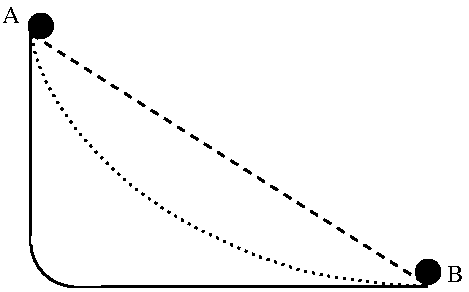
\includegraphics[width=.35\textwidth]{image0201}
\caption{Comparison of three different paths: straight line (dashed), maximum initial acceleration path (continuous) and brachistocrone (dotted)}
\end{figure}
Under this condition Bernoulli asked himself, what is the shape of the ground so that the ball in A reaches B in minimum time?

Several possibilities can be considered:
\begin{enumerate} 
\item a straight line
\item something that goes down sharply and then reaches the target point with a straight line.
\end{enumerate}

Turned out that was neither of those: they are both slower than minimum time, which materializes with a brachistochrone curve.

So Optimal control is a framework that helps us answer questions such as: what is the trajectory that allows me to go from this place to another
\begin{itemize} 
\item in minimum time
\item consuming the minimum amount of energy
\item  reaching the maximum velocity possible at the end of the trajectory.
\end{itemize}

These kind of question where we want to find the best motion for doing something, and by best we mean that it maximizes a certain critiria.

Before we dive deep into what optimal control is all about let us clarify what is the difference between Optimal control and Reactive control:
\begin{enumerate}
\item One of the key feature of reactive control which we have seen so far is that it always assume that you have a reference trajectory that you want to track. But we have never answer the question how do we actually compute these reference trajectories?

There are some cases where those reference trajectories are basically given by the problem (e.g. robot that cuts a material with a laser, knowing the profile of the cut you automatically know the trajectory that the end-effector should follow), but there are many cases where it is not obvious what trajectory the robot manipulator should follow.

In all of those circumstances where there is no clear trajectory to follow Reactive control is not enough because it does not allow to choose a specific solution for this problem, on this aspect Optimal control is the superior tool to leverage.

\item In reactive control the performance of the system are measured using quantities such as rise time, overshoot and settling time. In Optimal control, instead, we can use many more criteria in order to optimize the quality of the motion (minimize the energy, maximize the speed, minimize the time taken to do the motion)
\item In optimal control since it is based in optimized it is really easy to handle constraints. Inequality constraints are commonly used to represent the limits of the system (current limits, friction cones, joint limits, torque limits).
\end{enumerate}


\begin{table}[!h]
\centering
\begin{tabularx}{\textwidth}{|X|X|}
\textbf{Reactive control}&\textbf{Optimal control}\\
\toprule
need reference trajectory& no need for reference trajectory\\
rise time&objective clearly specified throguh cost function\\
overshoot&\\
settling time&\\
hard to handle constraints (e.g. joint position limits) & can handle constraints
\end{tabularx}
\end{table}

\subsection{Optimal control problem (O.C.P.)}

An optimal control problem takes the form of a minimization problem, but it is not really a minimization problem:
\begin{empheq}[box=%
	\fbox]{gather*}
\minimize_{x(\cdot), u(\cdot)} \int_0^T l(x(t), u(t), t)\,dt + l_f(x(T))
	\end{empheq}
subject to:
\begin{itemize}
\item{\makebox[5cm]{$\dot{x}(t) = f(x(t), u(t), t)\quad \forall t \in [0,T]$\hfill}} (\side{dynamics})
\item{\makebox[5cm]{$x(0) = x_0$\hfill} }(\side{initial conditions})
\item{\makebox[5cm]{$g(x(t), u(t), t) \le 0 \,\,\qquad \forall t \in [0, T]$\hfill}} (\side{path constraints}), e.g. actuator limits
\end{itemize}
where:
\begin{itemize}
\item{\makebox[5cm]{$\int_0^T l(x(t), u(t), t)\,dt$\hfill} is the }\side{running cost}
\item{\makebox[5cm]{$l_f(x(T))$\hfill} is the }\side{terminal cost}
\end{itemize}

As said before this is not a standard minimization/optimization problem, but an optimal control problem because
\begin{itemize}
\item $x(\cdot), u(\cdot)$ are trajectories, i.e. infinite-dimensional objects.
\item the constraints of the problem are infinitely many, given that they must be valid for all instances in the range $[0, T]$.
\end{itemize}

\subsubsection{Example of OCP: Pendulum}
We can imagine a pendulum robot and we want him to reach the vertical position (i.e. $q = 0$), where $q$ is the angle between the pose of the robot and the desired pose.

\[\minimize_{x(\cdot), u(\cdot)} \int_0^T\,q(t)^2\,dt + q(T)^2\]
subject to:
\begin{itemize}
\item $I\,\ddot{q} = \tau + m\,g\,sin(q) \Rightarrow \M{\dot{q}\\\ddot{q}} = \M{\dot{q}\\I^{-1}(\tau + m\,g\,sin(q))}$
\item $q(0) = q_0$
\item $\dot{q}(0) = \dot{q}_0$
\item $q^{min} \le q(t) \le q^{max}\qquad\forall t \in [0,T]$
\item $\abs{\tau(t)} \le \tau^{max}\qquad \forall t \in [0,T]$
\end{itemize}

where
\begin{itemize}
\item $x \triangleq (q, \dot{q})$
\item $u \triangleq \tau $
\end{itemize}

\begin{minipage}{.6\textwidth}
However the formulation of the running cost will make the robot manipulator reach $q = 0\degr{}$ as fast as possible, and maybe it is not something that you want. For this reason, additional terms are also included in the running cost. e.g, 
\[\int_0^T (q(t)^2 + u(t)^2 + \dot{q}(t)^2)\,dt\]
\end{minipage}
\hfill
\begin{minipage}{.35\textwidth}
\centering
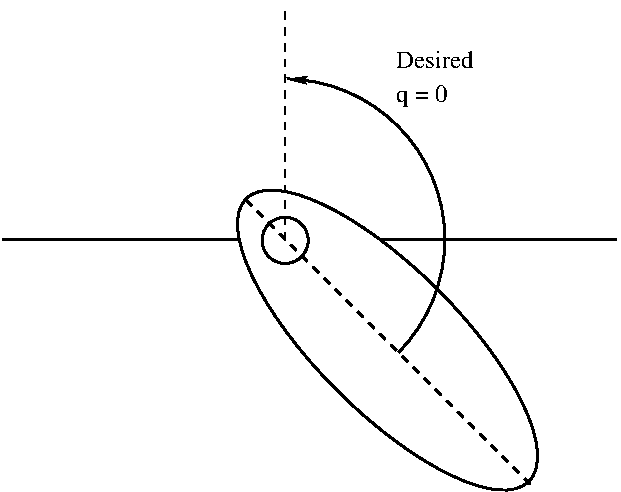
\includegraphics[width=.95\textwidth]{image0202}
\end{minipage}


\subsection{Optimal control method families}
There are many different approaches to solve a control problem. Some of them works in Continous Time, other in Discrete time, some of them are global and other are local.\newline

\begin{NiceTabular}[c]{lw{l}{5mm}l|cw{c}{51mm}c|cw{c}{51mm}c}
\hline
&&&\Block{1-3}{optimize $\Rightarrow$ discretize}&&&\Block{1-3}{discretize$\Rightarrow$optimize}&&\\
&&&\Block{1-3}{Continuous time}&&&\Block{1-3}{Discrete time}\\

\hline
&&&&&&&&\\
\Block{3-3}{Global}&&&\Block{3-3}{Hamilton-Jacobi-Bellman\\(HJB)}&&&\Block{3-3}{Dynamic Programming\\(DP)}\\
&&&&&&&&\\
&&&&&&&&\\
&&&&&&&&\\
\hline
&&&&&&&&\\
\Block{3-3}{Local}&&&\Block{3-3}{Pontryagin Maximum Principle (PMP)\\Calculus of variations\\Indirect methods}&&&\Block{3-3}{Direct methods}\\
&&&&&&&&\\
&&&&&&&&\\
&&&&&&&&
\end{NiceTabular}

\section{Dynamic Programming (DP)}
\subsection{Principle of optimality (Bellman)}
Dynamics Programming is based on the \side{principle of optimality}, aka the \side{Bellman principle}.

Let us suppose we have an optimal trajectory to go from one point to another. 
\begin{figure}[!h]
\centering
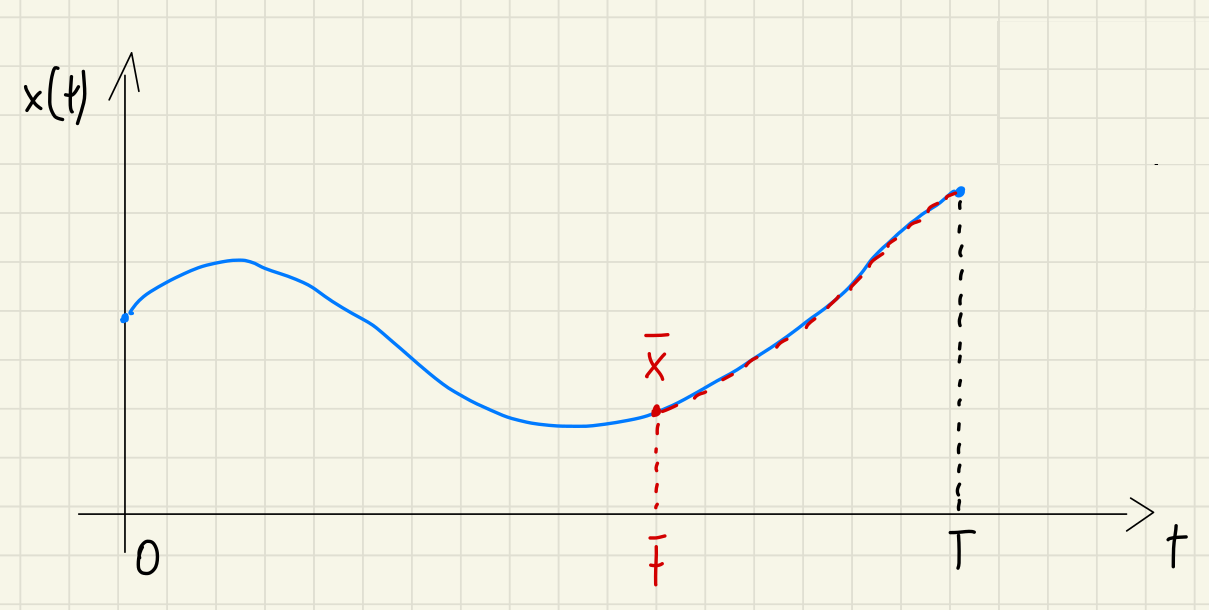
\includegraphics[width=.6\textwidth]{image0203}
\caption{Bellman optimality principle visual proof: if the continuous line is an optimal trajectory than the dotted subtrajectory is also optimal}
\end{figure}

What the principle of optimality says is that if you have an optimal trajectory then each subarc is in itself an optimal arc.

In other words, if the trajectory is the optimal trajectory in order to go from point A to point B, then no matter which initial point of the curve you start from the arc connecting such initial condition to the final point is the optimal trajectory.

This is rather trivial because if there is another arc that is the optimal trajectory to reach the final point than I could replace such arc to the original optimal trajectory, but since the original one is optimal by assumption that cannot be the case.

The principle of optimality can be used to simplify the solution of a discrete time optimal control problem.
\subsection{Dynamic Programming approach}

In dynamic programming the optimal control problem is assumed to be already in discrete time; that might be bacause we already have a discrete time problem (e.g. games, chess) or might be a continuous time problem that you discretized in time.

Therefore, the trajectories $x(\cdot)$ and $u(\cdot)$ are not in continuous time, but they are trajectories in discrete time (basically matrices).

The integral is replaced by a summation (equivalent of the integral).
\[\minimize_{X, U} \sum_{i=0}^{N-1} l(x_i, u_i)\]

The dynamics	that we have as a constraints are a discrete time dynamics.
subject to:
\begin{itemize}
\item $x_{i+1} = f(x_i, u_i)\qquad i = 0\,...\,N-1$
\item No terminal cost for sake of simplicity
\end{itemize}

To apply the principle of optimality to dynamic programming we need to split this problem into 2 parts.

Take M s.t. $0 \le M < N$. Then we split the problem cost:
\begin{gather}
\minimize_{X, U} \left[\sum_{i=0}^{M-1} \left( l(x_i, u_i) + I(x_{i+1} - f(x_i, u_i))\right) + \sum_{i=M}^{N-1}\left( l(x_i, u_i) + I(x_{i+1} - f(x_i, u_i))\right)\right]\\
\minimize_{X, U} \left[c_0(X_{1:M}, U_{0:M-1}) + c_M(x_M, X_{M+1:N}, U_{M:N-1})\right]
\end{gather}
In this formulation that constraint has been integrated in the cost function through the \side{Indicator function}. Such operator is zero when the input is zero and it is infinity otherwise.

Our constraints can now be seen as a high cost term if it is violated.

Now instead of doing the minimization of the sum of the two terms, since they depend on the different part of the trajectory (even though they both depend on $x_M$) I can treat them as decoupled and find the minimum of $c_M$, find the value of $x_M$ and lastly minimize $c_0$.

Formally:
\[\minimize_{X_{1:M}, U_{0:M-1}}\left[c_0(X_{1:M},U_{0:-1}) + \minimize_{X_{M+1:N}, U_{M:N-1}} c_M(x_M, X_{M+1:N}, U_{M:N-1})\right]\]
\[V_0(x_0) = \minimize_{X_{1:M}, U_{0:M-1}} c_0(X_{1:M}, U_{0:M-1}) + V_M(x_M)\]
We have still an optimal control problem, which parameters are still hidden inside $c_0$, but the big difference is that now we are optimizing over a smaller trajectory thanks to a separation of the problem formulation into two smaller minimization problems.

And since M can be chosen to be every value we want, we can repeat the same process as many times as we want and make the smaller problems to be optimizing over one value of the trajectory (i.e. one time step).

We therefore solve a sequence of problems: one for each time step, which simplifies drastically the original problem.

By iterating over we can get the optimal solution of the form:
\[V_i(x_i) = \minimize_{u_i}\left[l(x_i,u_i) + V_{i+1}(f(x_i,u_i))\right]\]
$V_M(x_M)$ can be interpreted as the optimal cost that we have to pay if we start from state $x_M$ at time M onward and behaving optimally. This function is called \side{Value function} or \side{Optimal cost-to-go}.

In conclusion:

Given a discrete-time finite-horizon OCP, we can initialize the dynamic programming algorithm writing the value function for the last time step
\[V_N(x_N) = l_f(x_N)\]
And then you use the recursive optimality principle (backward in time):
\[V_i(z) = \minimize_{u} l(z, u) + V_{i+1}(f(z,u))\qquad i = N-1,...,0\]
Once you have $V_i \,\,\forall i \in [0, N]$ you can compute the optimal control as:
\begin{empheq}[box=%
	\fbox]{gather*}
		u_i^*(x) = \argmin_u  l(x,u) + V_{i+1}(f(x,u))
	\end{empheq}



Observations:
\begin{itemize}
\item $u_i^*$ is not only an optimal control trajectory, but an \side{optimal feedback control policy}, because $u$ can be computed as function of $x$ so depending where we are in the state we get a different value of $u$.
\item The function to minimize is often called \side{Q function}.
\item the formulation of $V_i(z)$ is a \side{parametric optimization}, which is different from \side{numerical optimization}, because the result is not a value, but a function.
\end{itemize}

In summary:
\begin{enumerate}
\item Dynamic Programming is a global method, so it tries to get the global solution for a discrete time OCP.
\item The solution is not an open loop trajectory but it is a feedback control policy. So at every state and every time it tells you what the optimal solution is.
\item The main problem with dynamic programming is that it is applicable only in specific cases.
	\begin{enumerate}
	\item discrete state and control space. So the number of states and control inputs is bounded. (tipically not the case in robotics)
	In this scenario parametric optimization is replaced by numerical optimization applied to all possible states.
	
	The results are stored in a table called \side{lookup table}.
	
	The main disadvantage is the so called \side{Curse of dimensionality}. In fact, one may think, if we have a continuos robotic problem, can we discretize the state and the control space with a sufficiently fine grid. Yes, but the only problem is that if you want to discretize with a fine grid than you will get a very large state and control space (even if it is discrete).
	
	So suppose that you have a robot manipulator with 6 joints and you want to discretize the range of each joint both in position and velocity in 10 values. In this case you are going to have $10^{12}$ possible states which is a big number.
	
	The table that you are going to store in memory is of the same size, it has $10^{12}$ columns.
	
	So Dynamic programing is only applicable up to 2 to 4 states-control.
	
	However, in Dynamic programming it is easy to handle integer variables.
	\item Linear dynamics and quadratic cost function. In this case the problem that you have to solve is a \side{Linear Quadratic Regulator (LQR)}.
	
	The problem that we try to solve becomes a quadratic program that has a closed solution.
	\end{enumerate}
\item There are variants of Dynamic programming that go under the name of \side{Approximate Dynamic Programming} or \side{Neural Dynamic Programming} and those are basically Reinforcement Learning algorithms.
\end{enumerate}

\section{Direct methods}

\side{Direct methods} is a family of methods where there are different classes of methods, and the main difference w.r.t. Dynamic Programming is that they are local: i.e. they do not try to solve the problem for every possible state at every possible time and find the global optimum, but they just try to find a solution that is locally optimal.

It means that if you try to perturbe the solution you can only do worst.

\subsection{Introduction}

The key idea of Direct methods is really simple and intuitive.

Considering the following optimal control problem, which looks a lot like an optimization problem, you proceed to discretize the parameters of the problem. So you take the trajectory  and you parametrize such trajectory (e.g. with a polynomial) and obtain a finite number of parameters to represent this trajectory (e.g. coefficients of the polynomial).

In this way the number of decision variables is now finite.

The second problem related to the constraints (which are infinitly many) and you discretize em in time: i.e. you check the constraint at each time step (e.g. every 10ms).

The problem now becomes an optimization problem, so you can apply Newton Method to try to find the local solution.
 
However, the discretization process is not as simple as it sounds.

In summary:
\begin{itemize}
\item Discretize the Optimal control Problem and use a \side{non linear programming solver (NLP)} to find a local optimum.
\item The Discretization takes two steps:
\begin{enumerate}
\item Parametrize state and control trajectories (e.g. with polynomials).
\item Enforce constraints (both dynamics and path inequalities) on a grid.
\[t_0 < t_1 < t_2 < ... < t_N\]
Tons of theory/methods to choose trajectory parametrization and time grid so that NLP is a good approximation of OCP and \side{well conditioned} (a matrix is \side{ill-conditioned} if it has both very large and very small elements, in this conditioned it may occur loss of precision).
\end{enumerate}
\item There are three main families of Direct methods:
\begin{enumerate}
\item \side{Single Shooting} aka \side{Sequential approach}.
\begin{itemize}
\item Discretize only the control trajectory ($u(t)$).
\item Comput the state $x(t)$ integrating the dynamics.
\item No need to have dynamic constraints (you can omit the state as a control variable of the problem, because you can indirectly compute it from $u(t)$ and from the knowledge of the dynamics).
\end{itemize}
\item \side{Collocation} aka \side{Simultaneous approach}.
\begin{itemize}
\item Discretize both $x(t)$ and $u(t)$
\item Enforce the dynamics on a time grid. In this case you have to use the dynamics as a constraint to make sure since you have both $x(t)$ and $u(t)$ as decision variables, the solver chooses the state in a coherent way.
\end{itemize}
\item \side{Multiple Shooting}
\begin{itemize}
\item Discretize $u(t)$
\item Discretize $x(t)$ only at few points in time
\item Compute intermediate values of $x(t)$ by matter of integration
\end{itemize}
\end{enumerate}
\end{itemize}

\subsection{Single Shooting - Sequential Approach}
In single shooting you discretize the control $u(t)$ on a fixed grid $0 = t_0 < t_1 < ... < t_N = t_f$
\begin{figure}[!h]
\centering
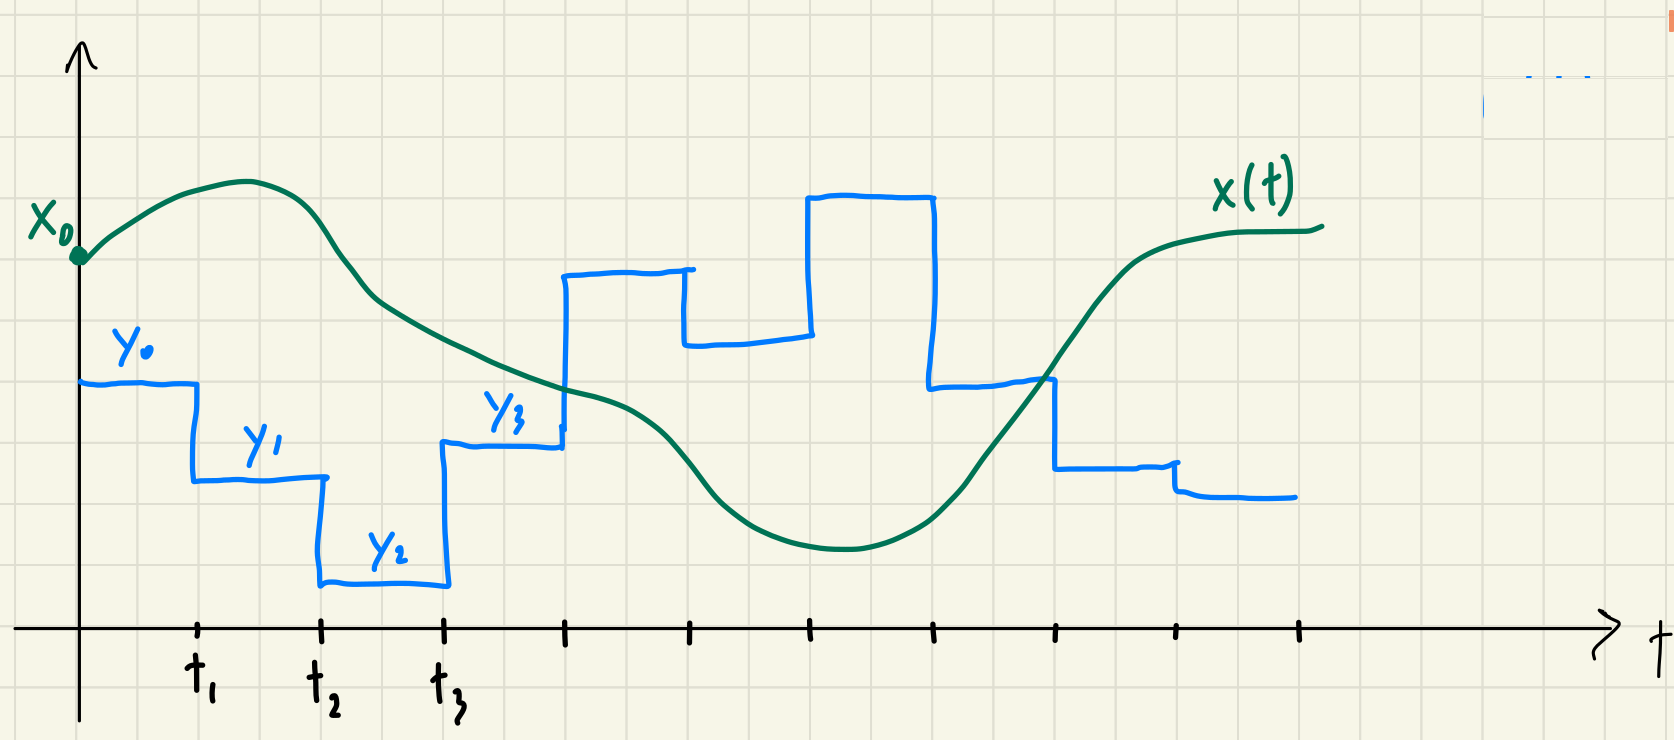
\includegraphics[width=.6\textwidth]{image0204}
\end{figure}

A very classical option for the discretization of the control is to do a piece-wise constant trajectory. So the control can only change at certain time and it remains constant.
\[u(t) = y_i \qquad\forall t\in[t_i, t_{i+1}]\]
You then proceed to compute $x(t)$ from $u(t)$ by integrating the dynamics
\begin{align*}
\dot{x} &= f(x,u,t)\\
x(0) &= x_0
\end{align*}

Of course the control can be discretize in other ways, but in practice this is what happends most of the time (e.g. piece-wise polynomial).

The non linear program that you get by using single shooting is:
\[\minimize_{y}\,\int_{0}^{t_f} \,l(x(t; y), u(t; y))\,dt \,+\,l_f(x(t_f; y))\]
subject to:
\begin{itemize}
\item{\makebox[5cm]{$g(x(t_i;y), u(t_i; y), t_i) \le 0$\hfill} $i=0 ... N$} are the \side{Discretized Path constraints}
\end{itemize}

The Running cost integral tipically is computed when integrating dynamics, and you do it by using an \side{augmented state}
\begin{gather*}
c(t) = \int_0^t l(\cdot, \cdot) \,dt\\
\begin{dcases}
\dot{c}(t) = l(\cdot, \cdot)\\
c(0) = 0
\end{dcases}
\end{gather*}
Given that we can define the augmented state $\bar{x}$ as:
\begin{gather*}
\bar{x} = (x,c)\\
\dot{\bar{x}} = \M{f(x,u,t)\\l(x,u)}
\end{gather*}

What we still need to do in order to implement a single shooting optimal control method are the computation of the sensitivities.
\subsubsection{Computing the sensitivities}

The \side{sensitivities} are the derivatives of the integration scheme that we are using to derive the state from the control.

Why do we need to differentiate between integration schemes? Because we are using an optimal optimization solver that requires the gradient of the cost function to work. So our cost function depends both on the state and the control, but actually the state depends itself on the control and this dependency is decided by the integration scheme that we are using.

So when we are computing the gradient of the cost function we need to take into account the gradient of the integration scheme, because to compute the cost function we need to evaluate the integration scheme.

This is not very difficult, it boils down to apply the chain rule in order to compute the derivatives of a function that it is itself a function of a variable, which is not the variable we want to differentiate, but an indirect dependency.
(in broad terms: we want to differentiate the cost function which depends on the state which once again depends on $u$)

There is an efficient way to conduct this computation which is tipically used to implement single shooting methods.\newline

Let us assume to have:
\begin{itemize}
\item Cost function and constraints of a single shooting NLP depend on $x$ and $u$
\item $x(t)$ us computed from $u(t)$ by matter of integration
\item $u(t)$ is discretized in a piecewise matter or alternative way

This means that given the generic dynamic equation:
\[\dot{x} =  f(x(t), u(t), t)\]
Assuming a piece wise constant discretization of the control $u(t)$ of the form:
\[u(t) = y_i\qquad\forall t \in [t_i, t_{i+1}]\]
we can reformulate the differential equation with the notion of the control variable discretization:
\[\dot{x} = f(x(t), y_i, t)\qquad\forall t \in [t_i, t_{i+1}]\]
\end{itemize}

Then we have a cost function (which is a function of $y$)
\[c(y) = \int_0^T l(x(t), u(t))\,dt + l_f(x(T))  \approx \sum_{i=0}^{N-1} l(x_i, y_i)\cdot h + l_f(x_N)\]
where the running cost integral is approximated with the Euler Method instead of using the augmented state. Tipically we are not required to be accurate in the computation of the running cost, but we have to be accurate during the computation of the dynamics.

We obtained our cost that we would like to differentiate, i.e. we want to compute:
\[
\td{c}{y} =  \sum_{i=0}^{N-1}\,\td{l(x_i, y_i)}{y}\cdot h + \td{l_f(x_n)}{y}
\]

In order to do so we need to compute the two unique differentiation in the above formulation
\begin{itemize}
\item $l$ depends on $y$ directly (because is a function of $y$) but it also depends on $y$ indirectly (because is a function of $x$ that you obtain by integrating the dynamics using $y$ as a control input).

Therefore we need to take care of both dependencies
\begin{align*}
\td{l}{y} &= \pd{l}{x_i}\,\td{x_i}{y}  + \pd{l}{y}
\end{align*}
\item For the second term we only have the indirect dependency because the final cost has no direct dependency from the control.
\begin{align*}
\td{l_f}{y} &= \pd{l_f}{x_N} \td{x_N}{y}
\end{align*}
\end{itemize}
From an analysis of the two expressions we can conclude that the partial derivatives of $l$ and $l_f$ are usually easy to compute, because they are just the derivatives of these functions (which is the running cost, that we decide as a designer of the optimal control problem) and it is tipically a simple function (e.g. quadratic function that penalizes the deviations of the state or the control from a given reference).

The total derivatives of the two expressions are less trivial to compute and they depend on the integration scheme. Their meaning is: how much a certain state is gonna change if I modify my control input (considering the whole trajectory of control inputs, not a single control input).

From this observations we can conclude that the partial derivatives are vectors whereas the total derivative are matrices.

We will now look into how to compute the $\td{x_i}{y}$ terms.

Let us introduce the \side{integrator function} $\Phi$, which is the \side{discretized dynamics function}, such that:
\[x_{i+1} = \Phi(x_i, y_i)\qquad\Rightarrow \qquad\td{x_{i+1}}{y} = \pd{\Phi_i}{x_i}\,\td{x_i}{y} + \pd{\Phi_i}{y}\]
This is basically what our integration scheme computes. We have derived a recoursive relationship that allows us to compute the term $\td{x_i}{y}$ for time $i+1$ if we know the value of that term  at the previous time step. 

However, we need to know the other two derivatives of the integrator function that will depend on our choice of integration scheme.

Note that:
\[\pd{\Phi}{y} = \left(\pd{\Phi_i}{y_0},...,\pd{\Phi_i}{t_{N-1}}\right)\]
where 
\[\pd{\Phi_i}{y_j} = 0\,\,\forall i\ne j\]

Two questions remain unanswered:
\begin{enumerate}
\item How do we initialize the computation? (i.e. what is the value of $\td{x_0}{y}$)

We can initialize the computation with 
\[\td{x_0}{y} = 0\]
Because the input only affect the future not the present, the initial condition does not depend on the choice of control input.
\item How do we compute the other two terms in the above expression?

This depends on the integration scheme that we are using. Let us review all the method that we have reviewed in Appendix\ref{sec:num}.
\begin{itemize}
\item \textbf{Explicit Euler}
Suppose $\Phi$ is explicit Euler (RK1), than:
\[\Phi(x,u) = x + h\,f(x,u)\]
where $f$ is the continuous time dynamic of the system.

\begin{align*}
\pd{\Phi}{x} &= I + h\,\pd{f}{x}\\
\pd{\Phi}{u} &= h\,\pd{f}{u}
\end{align*}
Of course we need the derivatives of the continuous time dynamics.
\item \textbf{RK4}
Suppose that $\Phi$ is RK4 integrator and $f(\cdot)$ is time independent.
\begin{align*}
k_1 &= f(x_i, y_i)\\
k_2 &= f(x_i+\cfrac{1}{2}hk_1, y_i)\\
k_3 &= f(x_i+\cfrac{1}{2}hk_2, y_i)\\
k_4 &= f(x_i+hk_3, y_i)\\
x_{i+1} &= x_i + \cfrac{h}{6}(k_1 + 2k_2 + 2k_3 + k_4) \triangleq \Phi_i(x_i, y_i)
\end{align*}

The sensitivity w.r.t. $x$ is:
\[\pd{\Phi_i}{x_i}=I+\cfrac{h}{6}\left(\pd{k_1}{x_i} + 2 \pd{k_2}{x_i} + 2\pd{k_3}{x_i} + \pd{k_4}{x_i}\right)\]
where:
\begin{align*}
\pd{k_1}{x_i} &= \left.\pd{f}{x}\right|_{x_i}&\\
\pd{k_2}{x_i} &= \left.\pd{f}{x}\right|_{x_{i2}}\left(I + \frac{1}{2}h\pd{k_1}{x_i}\right)& x_{i2} = x_i + \cfrac{1}{2}hk_1\\
\pd{k_3}{x_i} &= \left.\pd{f}{x}\right|_{x_{i3}}\left(I + \frac{1}{2}h\pd{k_2}{x_i}\right)& x_{i3} = x_i + \cfrac{1}{2}hk_2\\
\pd{k_4}{x_i} &= \left.\pd{f}{x}\right|_{x_{i4}}\left(I + \frac{1}{2}h\pd{k_3}{x_i}\right)& x_{i4} = x_i + \cfrac{1}{2}hk_3\\
\end{align*}
whereas the sensitivity w.r.t $y$ is:
\[\pd{\Phi_i}{y_i} = \cfrac{h}{6}\left(\pd{k_1}{y_i} + 2\pd{k_2}{y_i} + 2\pd{k_3}{y_i} + \pd{k_4}{y_i}\right)\]
\begin{align*}
\pd{k_1}{y_i}&=\left.\pd{f}{y}\right|_{xi}\\
\pd{k_2}{y_i}&=\left.\pd{f}{y}\right|_{x_{i2}} + \left.\pd{f}{x}\right|_{x_{i2}}\left(\cfrac{1}{2}h\pd{k_1}{y_i}\right)\\
\pd{k_3}{y_i}&=\left.\pd{f}{y}\right|_{x_{i3}} + \left.\pd{f}{x}\right|_{x_{i3}}\left(\cfrac{1}{2}h\pd{k_2}{y_i}\right)\\
\pd{k_4}{y_i}&=\left.\pd{f}{y}\right|_{x_{i4}} + \left.\pd{f}{x}\right|_{x_{i4}}h\pd{k_3}{y_i}
\end{align*}
\end{itemize}
\end{enumerate}


In summary:
\begin{itemize}
\item Remove $x$ from problem variables
\item Discretize $u(t) = y_i \qquad \forall t \in [t_i, t_{i+1}]$
\item Compute $x$ by integrating dynamics $\dot{x} = f(x,u)$
\item Since $x$ is computed by integrating the dynamics we do not need to have the dynamics as a constraint in the problem. i.e. remove dynamics from constraints of the problem
\item Tipically in single shooting you use a High-order integration scheme because it is more efficient
\item In any case, when you use an integration scheme you need to differentiate the integration scheme itself in order to compute the gradient of the cost and of the constraints. (Hardest part in the implementation)
\end{itemize}


\subsection{Collocation - Simultaneous Approach}
In collocation, we not only discretize the control input $u(t)$, but we also discretize the state $x(t)$ trajectory.

We are going to have many more decision variables in our problem, we are also gonna have many more constraints given that in this case we need to represent the dynamics of the system as a constraint in the problem.
However, this is not necessarily slower to solve even though we have so many variables and constraints.

Formally:
\begin{itemize}
\item We discretize $x(t)$, tipically with polynomials (e.g. order k=0, piece-wise constant) on fine grid (i.e. the time between two successive steps is going to be small) which defines how accurate the representation of the dynamics is.
\[x(t) = s_i\qquad\forall t \in [t_i, t_{i+1}]\qquad\text{One polynomial for each time interval}\]
This was not the case for single shooting where you could take a large step size and use an high-order integration scheme to retrieve an accurate integration of the dynamics.
\item Replace the dynamics $\dot{x} = f(x,u)$ with:
\[\cfrac{s_{i+1} - s_i}{t_{i+1} - t_i} - f\left(\cfrac{s_{i+1} + s_i}{2}, y_i\right) = 0\qquad\qquad i=0, ... , N-1\]
The first fraction is an approximation of $\dot{x}$, whereas the $\cfrac{s_{i+1} + s_i}{2}$ is an approximation of $x$.
This formulation can be interpreted as a constraint that relates $s_{i+1}$ with $s_i$ and $y_i$, i.e.:
\[c(s_{i+1}, s_i, y_i) = 0\]
\item Approximate the cost integral:
\[\int_{t_i}^{t_{i+1}}\,l(x(t), u(t))\,dt \approx l\left(\cfrac{s_i + s_{i+1}}{2}, y_i\right)\,(t_{i+1} - t_i) \triangleq l_i(s_i, s_{i+1}, y_i)\]
It is not exactly an Euler integration scheme, but it is quite similar.
\end{itemize}

We can now write down the complete problem to see how it looks like.

\[\minimize_{s, y} \,\sum_{i=0}^{N-1}\,l_i(s_i, s_{i+1}, y_i) + l_f(s_N)\]
subject to:
\begin{itemize}
\item $s_0 - x_0 = 0$
\item $c_i(s_i, s_{i+1}, y_i) = 0\qquad i= 0, ..., N-1$
\item $g_i(s_i, y_i, t_i) \le 0\qquad i= 0, ..., N$ 
\end{itemize}

This problem has a very important feature which is \side{sparsity}, (e.g. a matrix is sparse if it has a lot of zeros inside), i.e. the gradient, the jacobian, the hessian of the problem (so the derivatives of cost function and constraints) are sparse matrices and vectors.

It is important because if you have a sparse problem and you use a solver that it is able to exploit the sparcity then it can be solved much more efficiently than if you just neglet the sparcity.

Why can we say  that this problem formulation is sparse?  What is the feature that gives away the sparsity?
For instance from the constraint: $c_i(s_i, s_{i+1}, y_i) = 0$, we can deduct that the Jacobian will be sparse

The sparsity is given to this term by the dependency of some limited variables, in other terms the constraint does not depend on all the variables. In this case when we are going to compute the derivative of the constraint w.r.t. all the variables, many of them will be zero.

The same concept applies to the cost function (dependency on a subset of all the variables). For this term the hessian will be sparse (however the gradient will not be sparse).

\subsection{Multiple shooting}
Multiple shooting it is a middle ground between collocation and single shooting.

\begin{itemize}
\item Discretize the control $u(t)$ on a \side{coarse grid} $t_0 < t_1 < ... < t_n$
\[u(t) = y_i \qquad\forall t \in [t_i, t_{i+1}]\]
\item Integrate numerically ODE in each interval $[t_i, t_{i+1}]$, starting from a state variable $s_i$:
\begin{align*}
\dot{x}(t) &= f(x_i(t), y_i)\qquad\qquad t\in [t_i, t_{i+1}]\\
x_i(t_i) &= s_i
\end{align*}
\item Obtain $x_i(t)$ and Numerically compute the integrals:
\[l_i(s_i, y_i) = \int_{t_i}^{t_{i+1}}\,l(x_i(t), y_i)\,dt\]
\end{itemize}
So in multiple shooting you have the control input discretized as in single shooting, but you also have some state variables and this is the main difference between the two approaches.

Contrary to Collocation where you have the state variable on a fine grid, here you have the state variables on a coarse grid, that guarantees very few state variables.

The remaining values of the states inbetween this state variables will be computed by matter of numerical integration.

What can happen in multiple shooting is that the result of the integration does not match with the value of the state variable that you have at the end, so extra contraints needs to be formulated to guarantee continuity of the state trajectory. The problem formulation then becomes:

\[\minimize_{s, y} \,\sum_{i=0}^{N-1}\,l_i(s_i, y_i)\,+\,l_f(x_N)\]
subject to:
\begin{itemize}
\item $s_0 - x_0 = 0$
\item $s_{i+1} - x_i(t_{i+1}, s_i, y_i) = 0\qquad$where $x_i(\cdot)$ is the result of numerical integration starting from $s_i$. And these type of constraints are called \side{continuity contraints}.
\item $g(s_i, y_i) \le 0$
\end{itemize}

\begin{figure}[!h]
\centering
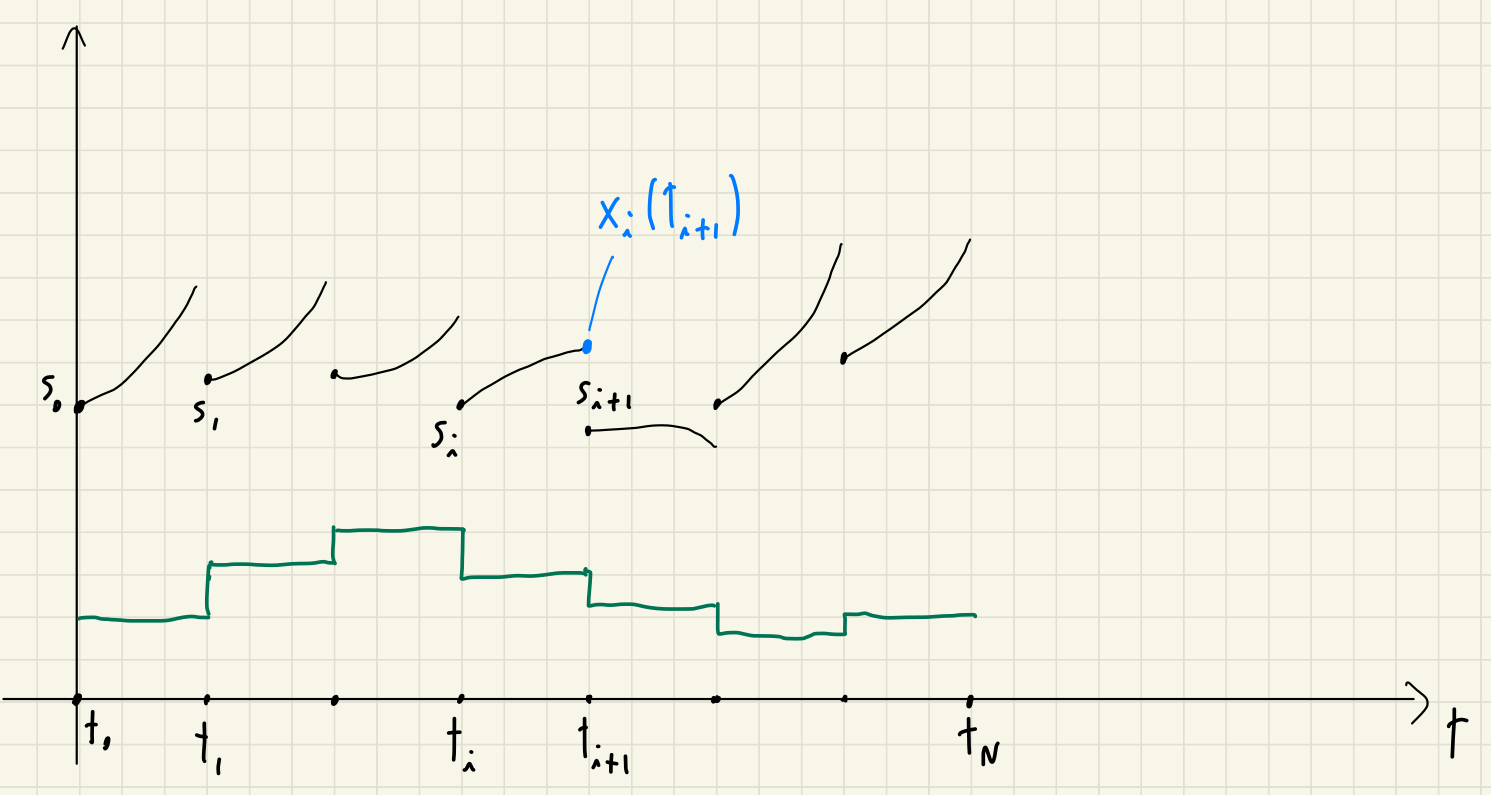
\includegraphics[width=.6\textwidth]{image0205}
\caption{Multiple shooting sketch}
\end{figure}

During the optimization problem the solver is allowed to have partial solution that have discontinuities and then the gaps will be collapsed to zero little by little. At the end of the solution problem we will obtain a continuous state trajectory.

This may seem like a bad property of the problem, but actually is what allows the solver to find better solutions most of the time.

In practical cases, Collocation and Multiple Shooting can find better solutions than Single Shooting.

 
\subsection{Comparison of Direct methods}
\begin{table}[!h]
\centering
\begin{tabularx}{\textwidth}{|X|X|X|}
\textbf{Single shooting} & \textbf{Multiple shooting} & \textbf{Collocation}\\
\hline
$\ooplus$ Small problem & $\oocirca$ Medium problem & $\oominus$ Large problem\\
$\ooplus$ Need only initial guess for $u(t)$ &$\ooplus$ Sparser than single shooting& $\oominus$ Cannot adapt time grid\\
$\ooplus$ Can use off-the shelp ODE solver &$\oominus$ Less sparse than collocation & $\ooplus$ Sparse problem\\
$\oominus$ Cannot exploit knowledge of $x$ in initialization & $\ooplus$ Unstable Ok &$\ooplus$ Work well with unstable systems\\
$\oominus$ ODE solution can depend very nonlinearly on $y$ & $\ooplus$ Initialize $x(t)$ & $\ooplus$ Can initialize $x$\\
$\oominus$ Numerical issues for unstable systems&&
\end{tabularx}
\end{table}
\section{Linear Quadratic Regulator (LQR)}
\side{Linear Quadratic Regulator LQR} is a method to solve a very specific kind of optimal control problem. What is special about this optimal control problem is that is  particularly simple because the dynamics is represented by a \side{discrete-time linear system}: 
\[x_{t+1} = A\,x_t + B\,u_t\]
And the objetive is to choose the control inputs $u_0, u_1, ...$ so that:
\begin{itemize}
\item $x$ is ``small'' $\Rightarrow$ good regulation/performance
\item $u$ is ``small'' $\Rightarrow$ small effort/energy consumption
\end{itemize}
These are usually competing objectives (you cannot have both at the same time) because if you keep $u$ very small than $x$ does whatever it wants, and tipically if you want to keep $x$ small you need some control effort.

So we need to find a trade-off between these two objectives, and that is what LQR does.

More precisely the LQR control problem takes the following form:
\begin{empheq}[box=%
\fbox]{gather*}
\minimize_{U} J(U) = \sum_{i=0}^{N-1} = (x_i^T\,Q\,x_i + u_i^T\,R\,u_i) + x_N^T\,Q_f\,x_N
\end{empheq}
subject to:
\begin{itemize}
\item $x_{i+1} = A\,x_i + B\,u_i\qquad i = 0, ..., N-1$
\end{itemize}
With a quadratic cost function, where$Q$ defines the quadratic form of the state, $R$ is the matrix that defines the quadratic form of the control and $Q_f$ defines the quadratic form of the final cost.

All the quadratics form are strictly positive definites (strinctly positive eigenvalues) or semi-positive definites (eigenvalues can be zero), i.e.
\begin{gather*}
Q = Q^T \ge 0\qquad;\qquad Q_f = Q_f^T \ge 0 \qquad;\qquad R=R^T > 0
\end{gather*}

As a consequence, any time that you have a state or a control that is not zero than you are increasing the cost. So idealy you would like to have all the variables at zero to achieve zero cost which is the minimum of the cost function (however that is not going to be possible).

The two knobs to tune the problem to achieve the behaviour of the system that you want are $Q$ and $R$, in particular:
\begin{itemize}
\item $Q$ large $\Rightarrow$ $x$ small is more important
\item $R$ large $\Rightarrow$ $u$ small is more important
\end{itemize}

The LQR optimal control problem can be rewritten in the following form
\[\minimize_{X, U} J(X, U) = \norma{\bar{Q}\,X}^2 + \norma{\bar{R}\,U}^2\]
subject to:
\begin{itemize}
\item $X = G\,U + H\,x_0$
\item with block diagonal matrices: 
\begin{gather*}
\bar{Q}\triangleq diag(Q^{\sfrac{1}{2}}, ..., Q^{\sfrac{1}{2}}, Q_f^{\sfrac{1}{2}})\qquad\text{and}\qquad \bar{R}\triangleq diag(R^{\sfrac{1}{2}}, ..., R^{\sfrac{1}{2}})
\end{gather*}
\end{itemize}
where we introduced the variables $X$ and $U$ containing the whole trajectory of the state and the control (discretized).

Also the dynamics can be written in linear form:
\begin{align*}
x_1 &= A\,x_0\,+\,B\,u_0\\
x_2 &= A\,x_1\,+\,B\,u_1\\
&\text{substituting the first expression into the second}\\
&= A^2\,x_0\,+\,AB\,u_0 + B\,u \\
x_3 &= A^3\,x_0 + A^2Bu_0 + ABu_1 + B\,u_2
\end{align*}
Iterating through each state we can represent the linear dynamics system in the matrix form:
\[
\begin{bNiceArray}{c}
x_1\\x_2\\\\\Vdots\\x_N
\end{bNiceArray}
=
\begin{bNiceArray}{c}
A\\A^2\\\\\Vdots\\A^N
\end{bNiceArray}
x_0+
\begin{bNiceArray}{ccccc}
B &&& &\\
AB & B &&&\\
 &\Vdots&\Ddots&&\\
\Vdots &&&&\\
A^{N-1}B&A^{N-2}B&\Cdots&&B
\end{bNiceArray}
\begin{bNiceArray}{c}
u_0\\u_1\\\\\Vdots\\u_{N-1}
\end{bNiceArray}
\]
So we can see that the state trajectory takes the following compact form:
\[X = H\,x_0 + G\,U\]

If we eliminate $X$ from the problem variables given the linear dynamic constraints, obtaining the new problem without constraints:
\begin{align*}
\minimize_{U}\,J(U) &= \norma{\bar{Q} (G\,U + H\,x_0)}^2 + \norma{\bar{R}\,U}^2\\
&= \left\lVert\M{\bar{Q}\,G\\\bar{R}} \,U + \M{\bar{Q}\,H\,x_0\\0}\right\rVert^2
\end{align*}
Now we can clearly see that the LQR optimal control problem is nothing more that a big \side{least-squares problem}, with dimension $N(n+m)\times Nm$ and cost $O(N^3nm^2)$ using Quadratic regulator.

where:
\begin{itemize}
\item $N$ is the length of the \side{horizon} (tipically quite large)
\item $n$ is the size of the state
\item $m$ is the size of the control
\end{itemize}

As a consequence, LQR gives us a more efficient way of computing the solution of the least square program by exploiting the structure of the program.

\subsection{LQR via Dynamic Programming}
LQR can be derived from the principle of Dynamic Programming.

Dynamic Programming is in general very difficult to apply to a real problem because you need to solve a parametric optimization problem. And LQR is one of those rare cases in which you can actually use Dynamic Programming, because the parametric optimization problem is a quadratic program (can be solved analytically).

We therefore proceed to write down the LQR problem definining the value function (optimal cost starting at a certain state, at a certain time):
\[V_t(z) = \minimize_{u_t = (u_t,...u_{N-1})} \sum_{k=1}^{N-1}(x_k^T\,Q\,x_k + u_k^T\,R\,u_k)\,+\,x_N^T\,Q_f\,x_N\]
subject to:
\begin{itemize}
\item $x_t = z$
\item $x_{k+1} = A\,x_k\,+\,B\,u_k\qquad\forall k = t, ..., N-1$
\end{itemize}
Therefore the value function $V_t(z)$ represent the optimal cost starting in $z$ at time $t$.

Of course the value function at time $0$ starting at state $x_0$ (i.e. $V_0(x_0)$) is nothing more than the optimal cost of the original problem.

The objective of Dynamic Programming is recursively minimize the value function starting at the last time step $N$ backwards.
The reason why we do so is because for the last time step we already know the value function, i.e. the terminal cost of the LQR problem:
\[V_N(z) = z^T\,Q_f\,z\]
From this point we can leverage the Bellman optimality equation that defines the value function at time $i$ as a function of the value function at time $i+1$ and apply this recursively going backward in time.
\[V_t(z) = \minimize_{w, U_{t+1}} z^TQz + w^TRw\,+\sum_{k=t+1}^{N-1}(x_k^TQx_k + u_k^TRu_k) + x_N^TQ_fx_N\]
subject to:
\begin{itemize}
\item $x_{k+1}=Ax_k+Bu_k$
\item $u_t = w$
\end{itemize}
Note that the value function above was split in the cost at time $t$ (left) and the cost starting from the $t$ going onwards until $N$.

The second part of the problem is nothing more than the value function at time $t+1$, i.e. $V_{t+1}(Az+Bw)$. So I can replace that part obtaining:
\[v_t(z) = \minimize_w z^TQz+w^TRw\,+\,V_{t+1}(Az+Bw)\]

NOTE: $Az + Bw$ is the next state i.e. $x_{t+1}$.

Now that we obtained the recursive optimality equation we can initialize it with the quadratic form for time $N$ and compute the value function recursively backward in time to see if it mantains this quadratic form or if it takes a  more complex form.

Assuming the $v_{t+1}$ is quadratic (that is true for $t+1 = N$), we can define the following quantities:
\begin{gather*}
V_{t+1}(z) = z^TP_{t+1}z\qquad\qquad P_{t+1} = P_{t+1}^T\ge 0 \qquad\qquad P_n=Q_f
\end{gather*}
And expand the minimization problem formulation with this new quantities
\begin{align*}
V_t(z) &= \min_w (z^TQz + w^TRw + V_{t+1}(Az+Bw))\\
&=z^TQz\,+\,\min_w(w^TRw\,+(Az+Bw)^TP_{t+1}(Az+Bw))\\
&=z^TQz\,+\,\min_w(w^T(R+B^TP_{t+1}B)w + 2z^TA^TP_{t+1}Bw) + z^TA^TP_{t+1}Az\\
&=z^T(Q+A^TP_{t+1}A)z + \min_w(\,(w^THw + 2g^Tw)\triangleq f(w)\,)
\end{align*}

where $H$ is the \side{Hessian of the quadratic form} and $g$ is the \side{gradient of the linear form}.

The minimization process is achieved by computing the gradient of the objective function to minimize (i.e. $f(w)$) and set it to zero:
\[\nabla f=2Hw+2g=0\]
which has solution:
\begin{align*}
w^* &= -H^{-1}g = -(R+B^TP_{t+1}B)^{-1}B^TP_{t+1}Az\\
&=K_tz
\end{align*}
Note that the matrix $H$ is always invertible by assumption: in fact, $R$ and $P_{t+1}$ are positive definite and their sum will always be a positive definite matrix, which is always invertible.

At this point we can compute $V_t(z)$ with the optimal value of the decision variable $w = w^*$.
\begin{align*}
V_t(z) &= z^T(Q+A^TP_{t+1}A)z + g^TH^{-1}\cancel{H}\cancel{H^{-1}}g -2g^TH^{-1}g\\
&=z^T(Q+A^TP_{t+1}A)z  - g^TH^{-1}g\\
&=z^T(Q + A^TP_{t+1}A - A^TP_{t+1}BH^{-1}B^TP_{t+1}A)z
\end{align*}
The result is a purely quadratic function in $z$ and the matrix inside is what we called $P_t$. By doing so we demonstrated that if the value function
\[V_{t+1}(z) = z^TP_{t+1}z\]
is purely quadratic at time $t+1$ than also the value function at time $t$ is purely quadratic, i.e.
\[V_t(z) = z^TP_tz\]
Therefore the value function is quadratic for all $t$ and we have a formulation of the value function at time $t$ starting from the value function starting at time $t+1$.

We can also prove that if the value function is positive semi-definite at time $t+1$ then also the value function at time $t$ will be positive semi-definite.

\begin{proof}
Given $P_{t+1}\ge0 , Q\ge0, R>0$ then $P_t\ge0$, which translates into proving that :
\[P_t = Q + AìTPA - A^TPB(R+B^TPB)^{-1}B^TPA\ge0\]
\begin{align*}
P-PB(R+B^TPB)^{-1}B^TP&\ge 0&\qquad S\triangleq P^{\sfrac{1}{2}}\Rightarrow P = SS^T\\
S(I-S^TB(R+B^TSS^TB)^{-1}B^TS)S^T&\ge0&\qquad L\triangleq R^{\sfrac{1}{2}}\Rightarrow R=LL^T\\
I-S^TB\left(\M{L&B^TS}\M{L^T\\S^TB}\right)^{-1}B^TS&\ge0&\qquad B^TS = \M{L&B^TS}\M{O_m\\I_n} = V\M{O_m\\I_n}\\
I-\M{0&1}V^T(VV^T)^{-1}V\M{0\\1}&\ge0&\qquad I = \M{0&1}\M{0\\1}\\
I-\M{0&1}V^{\dagger}V\M{0\\1}&\ge0&\\
\M{0&1}(I-V^{\dagger}V)\M{0\\1}&\ge0&\\
I-V^{\dagger}V&\ge0&
\end{align*}
Where the left hand side of the inequality is the \side{Projection matrix} (into nullspace of V) which eigenvalues are either 0 or 1 which implies that the inequality is always satisfied.
\end{proof}

Summary of the DP approach to solve the LQR problem:
\begin{enumerate}
\item Set $P_N = Q_f$ initialization of value function at time $N$ with the terminal cost.
\item For $t= N...1$, compute
\[P_{t-1} = Q + A^TP_tA - A^TP_tB(R+B^TP_tB)^{-1}B^TP_tA\]
\item For $t = 0...N-1$ compute the gain matrix
\[K_t = -(R+B^TP_{t+1}B)^{-1} B^TP_{t+1}A\]
\item For $t = 0...N-1$, compute the control input
\[u_t = K_t\,x_t\]
\end{enumerate}
You may notice that for this specific problem we actually not only recover the trajectory of optimal control inputs but we also have an optimal control policy given that $u_t$ is a linear function of the state. This gives us something more than an open-loop trajectory in contrast with the Direct methods (especially in Single Shooting).

The obtained \side{optimal linear feedback policy} can be used online on the real system: we can compute $u$ based on the current state, which might be different from what we would expect from the nominal plant (more useful in the presence of perturbations).

\subsection{Steady State Regulator}
Usually $P_t$ converges as $t$ decreases below $N$.

Steady-state value satisfies:
\[P_s = Q+A^TP_sA - A^TP_sB(R+B^TP_sB)^{-1}B^TP_sA\]
\side{Discrete-time algebraic Riccati Equation (DT-ARE)}
Can be solved by direct method or iterating RIccati recursion.

Therefore, for $t$ not close to $N$ we have constant feedback gain:
\[u = -(R+B^TP_sB)^{-1}B^TP_sA\]
\subsection{Time Varying System}
LQE is easily extended to Time Varying systems:
\[x_{t+1} =A_tx_t + B_tu_t\]
and Time Varying cost matrices:
\[\sum_{t=0}^{N-1}(x_t^TQ_tx_t + u_t^TR_tu_t) + x_N^TQ_fx_N\]
In this case there need not to be a steady-state solution though.
\subsection{Inhomogeneous system and costs}
\[\minimize \sum_{t=0}^{N-1}\M{x_t^T&u_t^T&1}\M{Q_t&S_t&q_t\\S_t^T&R_t&s_t\\q_t^T&s_t^T&0}\M{x_t\\u_t\\1} + \M{x_N^T&1}\M{Q_f&q_N\\q_N^T&0}\M{x_N\\1}\]
subject to:
\begin{itemize}
\item $x_{t+1} = A_tx_t + B_tu_t + c_t$
\item $x_0 = x^{init}$
\end{itemize}
Define augmented state $\bar{x} = \M{x&1}$
\begin{align*}
\M{x_{t+1}\\1} &=&\M{A_t&c_t\\0&1}&\M{x_t\\1} + &\M{B_t\\0}&u_t&\\
\bar{x}_{t+1} &= &\bar{A}_t &\bar{x}_t  + &\bar{B}_t &u_t&\Leftarrow \text{Homogeneous}
\end{align*}
\[J = \sum \M{\bar{x}_t^T&u_t^T}\M{\bar{Q}_t&\bar{S}_t\\\bar{S}_t^T&R_t}\M{\bar{x}_t\\u_t} + \bar{x}_N^T\bar{Q}_f\bar{x}_N\]
with:
\begin{gather*}
\bar{Q}_t\triangleq \M{Q_t&q_t\\q_t^T&0}\qquad\bar{S}_t\triangleq\M{S_t\\s_t^t}
\end{gather*}

The only difference is cross term $x^TSu$ in cost function.
DP solution easily extended.

Fin doptimal fedback policy for augmented system:
\[u=\bar{K}\bar{x} = \M{K&k}\M{x\\1} = Kx+k\]
Why inhomogeneous systems and costs:
\begin{itemize}
\item Tracking problems
\item Linearization of nonlinear systems
\item Filtering problems (e.g. Kalman)
\end{itemize}

\subsection{Tracking problems}
\[J = \sum_{t=0}^{N-1} (x_t-\bar{x}_t)^TQ(x_t-\bar{x}_t) + (u_t-\bar{u}_t)^TR(u_t-\bar{u}_t)\]
$\bar{x}, \bar{u}$ = reference trajectories to track.

Can be rewriteen as \side{inhomogeneous cost}:
\begin{align*}
J&=\sum x^TQx + u^TRu - 2\bar{x}^TQx - 2\bar{u}^TRu\\
&=\sum \M{x^T&u^T&1}\M{Q&0&Q\bar{x}\\0&R&R\bar{u}\\\bar{x}^TQ&\bar{u}^TR&0}\M{x\\u\\1}
\end{align*}

\subsection{Differential Dynamic Programming (DDP)}
\side{Differential Dynamic Programming (DDP)} is in some sense an extension of LQR, that handles \side{non-linear dynamical system}s and also \side{non-linear cost function}s.
This is a method that can be applied to a much more generic kind of optimal control problems, which takes the form:
\[\minimize \sum_{t=0}^{N-1}\,l_t(x_t, u_t) + l_N(x_N)\]
subject to:
\begin{itemize}
\item $x_{t+1} = f(x_t, u_t)$
\item $x_0 = x^{init}$
\end{itemize}
It is not completely a generic control problem because we do not have inequality constraints or any other type of constraints beside the dynamics. But surely more generic than Direct Methods, given that we can handle non linearities.

The idea of DDP vaguely resemble the approach of Newton Method and Numerical Optimization methods.

Start with a guess for the decision variable of the problem $U$ and alternate between the following three steps:
\begin{enumerate}
\item Linearize around current trajectory
\item Solve LQR to get variation of $U$
\item Line search to ensure convergence
\end{enumerate}
This is just an euristic, there is no guarantee of convergence, sometimes it will converge to the global optimum and sometimes it will converge to a local optimum.

The idea it remains the same, i.e. apply dynamic programming, but since you cannot really apply DP to the original system, you apply it to a linearization (aka local approximation) of the system
\begin{gather*}
V(z,i) =\minimize_{U_i} J_i(z, U_i)\qquad \text{where:}\quad U_i = (u_i, ... , u_{N-1})
\end{gather*}
We can subsequently apply Bellman optimality principle in order to split the cost in two parts:
\begin{align*}
V(z,i) &= \minimize_w\left[l_i(z,w) + V(f(z,w), i+1)\right] = \min_w Q(z,w)\\
Q(\bar{x} + z, \bar{u}+w)&\approx Q(\bar{x}, \bar{u}) + \M{Q_x^T&Q_u^T}\M{z\\w} + \cfrac{1}{2}\M{z^T&w^T}\M{Q_{xx}&Q_{xu}\\Q_{xu}^T&Q_{uu}}\M{z\\w}
\end{align*}

Since we do not really know how to minimize a non linear function we can take a quadratic approximation (via Taylor expansion) and minimize it.

where:
\begin{gather*}
Q_x\triangleq \pd{Q}{x}\qquad Q_u\triangleq\pd{Q}{u}\qquad Q_{xx}\triangleq\pdd{Q}{x}\qquad Q_{uu}\triangleq\pdd{Q}{u}\qquad Q_{xu}\triangleq \pd{Q_u}{x}
\end{gather*}
Once defined the derivative of the value function as follows:
\[V' \triangleq V(\cdot, i+1)\]
We can expand the partial derivatives, using the chain rule:
\begin{align*}
Q_x &= l_x + f_x^T V'_x\\
Q_u &= l_u + f_u^T V'_x\\
Q_{xx} &= l_{xx} + f_x^T V'_{xx}f_x + V'_x f_{xx}\\
Q_{uu} &= l_{uu} + f_u^T V'_{xx}f_u + V'_x f_{uu}\\
Q_{xu} &= l_{xu} + f_x^T V'_{xx}f_u + V'_x f_{xu}
\end{align*}

Moreover the quadratic cost function takes the following compact form:
\begin{align*}
Q(\bar{x}, \bar{u}) &= l(\bar{x}, \bar{u}) + V'(f(\bar{x}, \bar{u}))\\
\bar{Q} &= \bar{l} + \bar{V}'
\end{align*}

The DDP problem is reduce to minimizing the local quadratic model of $Q$. In doing so we get:
\[w^* = \argmin_w Q(z, w) = -Q_{uu}^-1 (Q_u + Q_{ux}\,z)\]
This expression is a bit more complicated than what we had before with LQR because it is not a purely linear function of the state, but it is an affine function of the state (Bias/constant term $Q_u$ and linear term $Q_{ux}z$).
The reason why it is not purely linear is because the cost is not purely quadratic but you have also the affine term (i.e. Linear terms).

Substituting $w^*$ inside the definition of the local approximation of the Q function $Q$ to recover the value function at the previous time step $V$, i.e.:
\begin{align*}
V &= \bar{Q} + Q_x^Tz + Q_u^Tw^* + \cfrac{1}{2}z^TQ_{xx}z + \cfrac{1}{2}{w^*}^TQ_{uu}w^* + z^TQ_{xu}w^*\\
&= \bar{Q} + (Q_x^T - Q_u^TQ_{uu}^{-1}Q_{ux})z + \cfrac{1}{2}z^T(Q_{xx} + \cancel{Q_{xu} Q_{uu}^-1 Q_{ux}} - \cancel{2}Q_{xu}Q_{uu}^{-1}Q_{ux})z + \\
& \qquad\qquad\cancel{Q_u^TQ_{uu}^{-1}Q_{ux}z} - \cancel{z^TQ_{xu}Q_{uu}^{-1}Q_u} + ...\\
&= \Delta V + V_xz + \cfrac{1}{2}z^TV_{xx}z
\end{align*}
where:
\begin{itemize}
\item $V_x \triangleq Q_x - Q_{xu}Q_{uu}^{-1}Q_u$
\item $V_{xx}\triangleq Q_{xx}-Q_{xu}Q_{uu}^{-1}Q_{ux}$
\item $\Delta V = \bar{Q} - \cfrac{1}{2} Q_u^T Q_{uu}^{-1} Q_u$
\end{itemize}

Once again what we just observed is that the value function starting from a quadratic approximation of the value function, if we propagate it backward in time using Bellman optimality equation, we still get a quadratic approximation of the value function for time $t-1$.

By applying this principle iteratively we always maintain a quadratic form of the value function.

There is one small detail: when we are working with a non linear system (that you do not need to worry about in the LQR problem given the initial assumption).
The matrix $Q_{uu}$, which we need to invert in order to compute the optimal control inputs, might not be invertible.

The way this is tipically handled is to introduce \side{regularization}:
\[\bar{Q}_{uu} = Q_{uu} + \mu\,I\]
where $\mu$ is the \side{regularization value}. If this value is sufficiently large that you can be sure that the new regularized matrix will always be invertible.

You can then replace the inverse of $Q_{uu}$ with the regularized version:
\begin{gather*}
w^* = -\bar{Q}_{uu}^{-1}(Q_u + Q_{ux}z) = \bar{w} + Kz \qquad \bar{w} \triangleq - \bar{Q}_{uu}^{-1}Q_u \qquad K \triangleq - \bar{Q}_{uu}^{-1}Q_{ux}
\end{gather*}

Substituting $w^*$ inside Q to get the value function, you get:
\begin{align*}
V &= \bar{Q} + Q_x^T z + Q_u^Tw^* + \cfrac{1}{2}z^TQ_{xx}z + \cfrac{1}{2}{w^*}^TQ_{uu}w^* + z^TQ_{xu}w^*&&\\
&=\bar{Q} + Q_u^T\bar{w} + (Q_x^T + Q_u^TK)z + \cfrac{1}{2}z^T(Q_{xx} + K^TQ_{uu}k + 2Q_{xu}K)z + \bar{w}^TQ_{uu}Kz &&\\
&\qquad\qquad+ \cfrac{1}{2}\bar{w}^TQ_{uu}\bar{w} + z^TQ_{xu}\bar{w}&&\\
&= \quad \bar{Q} + Q_u^T \bar{w} + \cfrac{1}{2}\bar{w}^TQ_{uu}\bar{w}&\Leftarrow&\Delta V\\
& \quad+(Q_x^T +Q_u^TK + \bar{w}^TQ_{uu}K + \bar{w}^TQ_{xu}^T)z&\Leftarrow &V_x\\
&\quad+\cfrac{1}{2}z^T(Q_{xx} + K^TQ_{uu}K + 2Q_{xu}K)z&\Leftarrow &V_{xx}
\end{align*}

Summary of the DDP algorithm:
\begin{enumerate}
\item Given an initial guess for the optimal control trajectory $\bar{U}$, compute the state trajectory $\bar{X}$ by matter of forward simulation in time $\dot{x} = f(x,u)$
\item \side{Backward Pass} (it is called this way because we have a loop backward in time):
\begin{enumerate}
\item Initialize the derivatives of the value function with the derivatives of the terminal cost, ie.e
\[V_x(N) = \nabla_xl_N\qquad\qquad V_{xx}(N) = \nabla_{xx}l_N\]
\item Loop backward in time ($i = N-1, ..., 0$)
\begin{itemize}
\item Compute the derivatives of the Q function, i.e. $Q_x, Q_u, Q_{xx}, Q_{uu}, Q_{xu}$
\item Compute the optimal control input 
\[w^* = -\bar{Q}_{uu}^{-1}(Q_u + Q_{ux}z) = \bar{w} + Kz\]
\item Compute the value function at time $i$, i.e. $V_{x}(i), V_{xx}(i)$
\end{itemize}
\end{enumerate}
\item \side{Forward Pass}, since you do not the state yet, we cannot compute the control input. Basically we need to do a line search.
\begin{enumerate}
\item set $\alpha = 1$. Which translate into taking a full step.
\item Simulate with 
\begin{align*}
u&=\bar{u} + w\\
&= \bar{u} + \alpha\,\bar{w} + K(z)\\
&= \bar{u} + \alpha\,\bar{w} + K(x - \bar{x})
\end{align*}
\item If cost has not decreased enough, you decrease $\alpha$ and repeat the previous step
\item Assign $\bar{x} = x$ and $\bar{u} = u$
\item If the forward pass has not converged repeat the Backward Pass, around the new trajectory $\bar{U}$.
\end{enumerate}
\end{enumerate}

In the end you obtain:
\begin{enumerate}
\item Optimal open-loop control $\bar{u}$
\item Locally optimal linear feedback gains $K$
\end{enumerate}
Which can be summarized in the feedback control policy (locally optimal)
\[u = \bar{u}+ K(x-\bar{x})\]

\subsubsection{How much should the cost decrease?}

It depends on $\alpha$, because if $\alpha$ is very small we cannot expect a big improvement in the cost because we are changing the control input by a small amount, whereas if $\alpha$ is large we can expect a larger improvement.
The idea is the same that we presented with Newton Method in line search, i.e. you compute how much you expect the cost to improve if your approximation of the function that you are minimzing is exact. And this will give you a baseline to compare against how much the cost is actually decreasing.

To compute how much the cost should decrease you need to take a look at the variation of the value function starting from the value function at time 0 for $z = 0$:
\begin{align*}
V_0(0) = \Delta V_0 &= \alpha \sum_{i=0}^{N-1}\bar{w}_i^T Q_{u,i} + \cfrac{\alpha^2}{2} \sum_{i=0}^{N-1}\bar{w}_i^TQ_{uu,i}\bar{w}_i + \sum_{i=0}^N\bar{l}_i\\
&=\alpha \sum_{i=0}^{N-1}\bar{w}_i^T Q_{u,i} + \cfrac{\alpha^2}{2} \sum_{i=0}^{N-1}\bar{w}_i^TQ_{uu,i}\bar{w}_i + J(\bar{U})\\
\Delta V_i &= \alpha \bar{w}_i^T Q_{u,i} + \cfrac{\alpha^2}{2}\bar{w}_i^T Q_{uu,i} \bar{w}_i + \Delta V_{i+1} + \bar{l}_i
\end{align*}
Here you can see that $\alpha$ appears both linearly  and quadratically.

Hence the expected cost improvement takes the form:
\[\Delta J(\alpha) = \Delta V_{0} - J(\bar{U})=\alpha d_1 + \cfrac{\alpha^2}{2}\,d_2\]
That means that every time I change $\alpha$ in the forward pass I do not need to recompute $d_1$ and $d_2$, but I only need to recompute $\Delta J(\alpha)$.

What is tipically done is:
\[\cfrac{J(U) - J(\bar{U})}{\Delta J(\alpha)}>c_1\]
You compute the real improvement (numerator) and the expected improvement (denominator) and finally accept this step if the ratio between the two is greater than a certain value (smaller than 1).

The parameter $c_1$ is an \side{hyperparameter} of the problem that you have to tune by hand.

\subsubsection{Regularization}
How do we tune the regularization value $\mu$.

In fact if this parameter is too small it will happen that:
\begin{itemize}
\item $\bar{Q}_{uu}$ may be singular
\item $\bar{w}$ may be too large, which results in very large control inputs. In this situation the local quadratic model may no longer be accurate with resulting small cost improvements
\end{itemize}
On the other hand if this parameter is too large then $\bar{w}$ may be too small and the convergence will be too slow.

Therefore the \side{Regularization Scheme} that we are going to follow is:
\begin{itemize}
\item If $\bar{Q}_{uu}$ is not invertible or $\cfrac{J(\bar{U}) - J(U)}{\Delta J(\alpha)}<c_2$, then we will increse the regularization factor
\item otherwise we will decrease the regularization factor, in order to speed up the convergence.
\end{itemize}


In Summary:

\begin{itemize}
\item DP gives us an efficient algorithm to solve LQR
\item The solution of LQR yields a \side{globally optimal feedback policy}
\item Extension to non linear systems (DDP)
\begin{itemize}
\item efficient recursive algorithm
\item no guarantees of convergence
\item can only find local optimum
\item feedforward + feedback policy
\item many hyper-parameters for regularization/line search $c_1, c_2, \mu, k_{\mu}, K$
\end{itemize}
\end{itemize}


\section{Model Predictive Control (MPC)}
\side{Model Predictive Control (MPC)} is a very popular technique used in many robotic systems and other fields outside robotics. 

Moreover, this particular control method connects what we have seen in reactive control and optimal control, because what we have seen so far in optimal control is just a mean of computing a trajectory and then using reactive control we can track the reference trajectory. 

With MPC we are unifying these 2 problems and solutions, because the idea of MPC is to use optimal control not only for computing the reference trajectory, but also to design the real time control loop (aka stabilizing the system).

We took a glimps of this type of approach in DDP, because DDP does not only yield the control trajectory but also the feedback gains: this allows us to the result of DDP as a feedback controller. However this is really specific to DDP since it is the only method that gives us the feedback gains (i.e. something to stabilize the systems).

All the other methods, such as Direct methods, only yield a control trajectory not the feedback gains, so in order for them to work they need to be coupled with a reactive controller.

Why do we need something else to do the stabilization? Mainly because we will always have uncertainty in the system, so even if you plan for an optimal trajectory, you cannot hope that you apply this control and the system would behave exactly as planned, you always need a feedback to stabilize the system.

In MPC we are trying to get rid completely of the reactive controller and use the optimal controller also to stabilize the system. The principle behind this method goes as follow:

Solve a \side{finite-horizon} OCP using the current state (that you measure or estimate) as initial state. Under this condition the optimal control problem takes the form:
\[X^*, U^* = \argmin_{X,U} \sum_{k=0}^{N-1} l(x_k, u_k)\]
subject to
\begin{itemize}
\item $x_{k+1} = f(x_k, u_k, k)\qquad\qquad k=0,...,N-1$
\item $x_{k+1}\in\mathfrak{X}, \quad u_k\in\mathfrak{U}\qquad\qquad k = 0,...,N-1$
\item $x_0 = x^{meas}$
\end{itemize}
The process to follow is:
\begin{enumerate}
\item Solve the optimal control problem
\item Obtain the optimal state trajectory and optimal control trajectory 
\item Take the first value of the optimal control trajectory $u_0$, and apply it
\item In the next iteration of the control loop, repeat the same process we the value of the optimal control input obtained in the previous step.

Of course you consider the initial state as the state measured or estimated in the current iteration.
\end{enumerate}

By solving the optimal control problem at each iteration you are always behaving in a optimal way because you are re-optimizing the trajectory based on the real state of the system not based on where you thought your system is according to your model.

The main problem of MPC comes from the difference between the trajectory that you predict whe you solve the OCP and the trajectory that you actually going to follow with your real system (this point does not take into account the presence of disturbances). Even if you do not have any disturbance, the trajecory that you are going to predict with the optimal control problem and the one that you are going to get with the MPC are going to be different.

The reason is because we are re-optimizing the trajectory at each step with an unseen point w.r.t. the previous optimization.
\begin{figure}[!h]
\centering
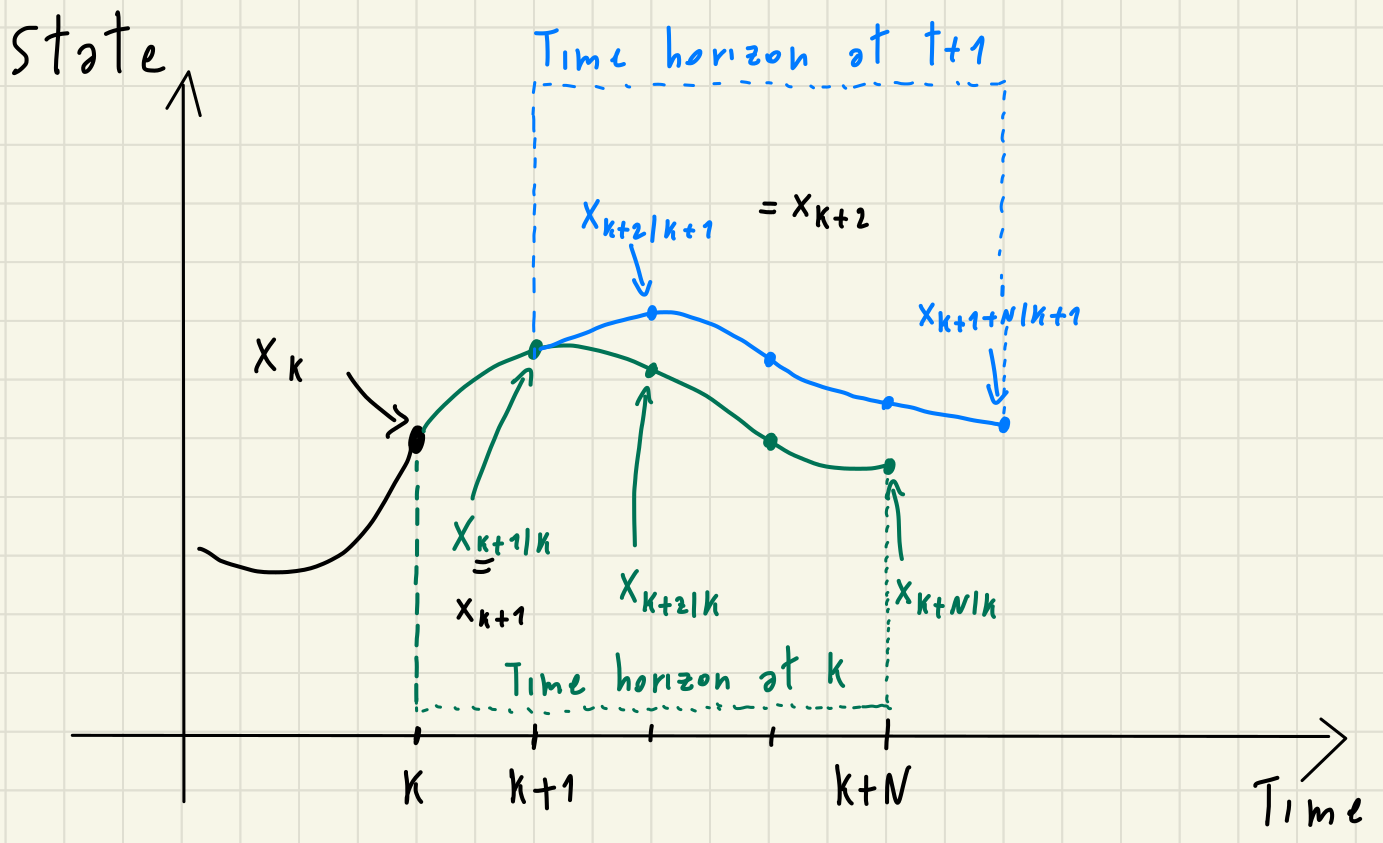
\includegraphics[width=.6\textwidth]{image0206}
\caption{First two iteration of a generic MPC: the real trajectory differs from the computed ones due to the fact that the algorithm re-optimize the trajectory on a different set of states}
\end{figure}

In other terms
\begin{itemize}
\item the OCP at time $k$ and $k+1$ optimize over different horizons so it can result in different trajectories.
\item Even without disturbances, predicted and actual trajectories can be different
\item What if at time $k+1$ I shorten the horizon to $N-1$? 

In this case the trajectory would be the same due to Bellman optimality principle.
\end{itemize}

The three main challenges when dealing with MPC are: 
\begin{enumerate}
\item \side{feasibility}.

Can I ensure that the OCP is always feasible?

What can I do if it is not feasible?

This is a problem given that if the problem is not feasible than the solver will not be able to yield any solution and so you lack a control input to apply to the system.
\item \side{stability}.

Can I ensure that MPC stabilizes the system?

Because even if you are computing the trajectory that all converge to zero, maybe the real trajectory that system is performing is diverging.
\item \side{computation time}

Can I solve the OCP sufficiently fast?
\end{enumerate}

\subsection{Infinite-Horizon MPC}
What would happen if instead of having a finite horizon MPC, we had an horizon that is infinite?

If the horizon is infinite than the horizon that is seen by each OCP that you solve is the same since they all go to infinity. So you no longer have the problem that we have discussed before (i.e. the trajectory that you get when optimizing is different from the trajectory that you actually get on the real system), because at each iteration the OCP uses the same horizon and the trajectory will be the same at each optimization.

In short: in this case predicted and actual trajectories are the same, assuming no distrurbances.
This follows from Bellman's principle of optimality.

Having $N=\infty$, if cost $l(x,u) \ge \alpha\,\norma{x}\,\,\forall x,u$ for some $\alpha>0$ then 
\begin{enumerate}
\item Having a finite cost implies stability. From the condition of the cost we can infer that the the cost can only be finite only if the state (or its norm) goes to zero. 
\item Since predicted and actual trajectories are equal, I have \side{recursive feasibility} along the closed-loop trajectory.
\end{enumerate}

Even though this scenario is purely theoretical (in practice we cannot impose an infinite horizon), it helps us get the key idea of stability and recursive feasibility of MPC which is: try to mimic an infinite horizon problem by including a \side{terminal cost} and \side{terminal constraint} that mimic the effect that I would get with the infinite horizon (much like what we did with DP with the value function).

In other terms the terminal cost should be an approximation of the tail of my \side{infinite horizon running cost} and the terminal constraints should be an approximation of all the extra constraints I would get with an infinte horizon.

If we take the standard finite horizon OCP:
\[V^*_N(\bar{x}) = \minimize_U \sum_{k=0}^{N-1} l(x_k, u_k)\]
subject to:
\begin{itemize}
\item $x_{k+1} = f(x_k, u_k)\qquad k = 0,...,N-1$
\item $x_k\in\mathfrak{X},\quad u_k\in\mathfrak{U}\qquad k= 0,...,N-1$
\item $x_0 = \bar{x}$
\end{itemize}
In order to ensure fisibility and stability we can extend the formulation using a terminal cost and terminal constraints:
\[V^*_N(\bar{x}) = \minimize_U \sum_{k=0}^{N-1} l(x_k, u_k) + l_f(x_N)\]
subject to:
\begin{itemize}
\item $x_{k+1} = f(x_k, u_k)\qquad k = 0,...,N-1$
\item $x_k\in\mathfrak{X},\quad u_k\in\mathfrak{U}\qquad k= 0,...,N-1$
\item $x_0 = \bar{x}$
\item $x_N\in\mathfrak{X_f}$
\end{itemize}

The question remains: how can we choose $l_f(\cdot)$ and $\mathfrak{X}$?

\subsection{Feasibility}
When talking about feasibility we need to distinguish between two cases, because they are very different from each other:
\begin{enumerate}
\item \side{Input constraints only}

This case is always feasible, because $u$ is our decision variable so if your control set is not empty, you can always choose a point inside this set and always obtain a solution.
\item \side{Hard state constraints}

If $N< \infty$ there is no guarantee that OCP remains feasible, even in nominal case.

$N=\infty$ ensures feasibility, but OCP has infinitely many constraints.
\end{enumerate}

The \side{Maximum Output Admissible Set theory} states that $N<\infty$ is enough to enforce recursive feasibility, but it does not specify how long the horizon should be in order that this is guaranteed.

A better way to deal with this problem is to use the \side{Maximum Control Invariant Set} which is a set that can be used as a terminal constraint and this ensures \side{closed-loop convergence}, but it can reduce the \side{domain of feasibility}, i.e. starting from a state for your original problem would be feasible, by using the Maximum Control Invariant Set as a constraint, your problem might become not feasible (especially if the system is perturbed).

In practice, this is almost the best thing that you could do (if you can do it).

\subsubsection{Control Invariant Set}
A set $S$ is \side{Control Invariant} if once you are inside the set you can stay inside the set.

In mathematical term:
A set $S$ is control invariant if $\forall x \in S, \exists u\in \mathfrak{U}$ s.t. the next state $f(x,u)\in S$.

\begin{theorem}
If $\mathfrak{X}_f$ is control invariant then MPC will be recursively feasible.
\end{theorem}
Visual proof:
\begin{figure}[!h]
\centering
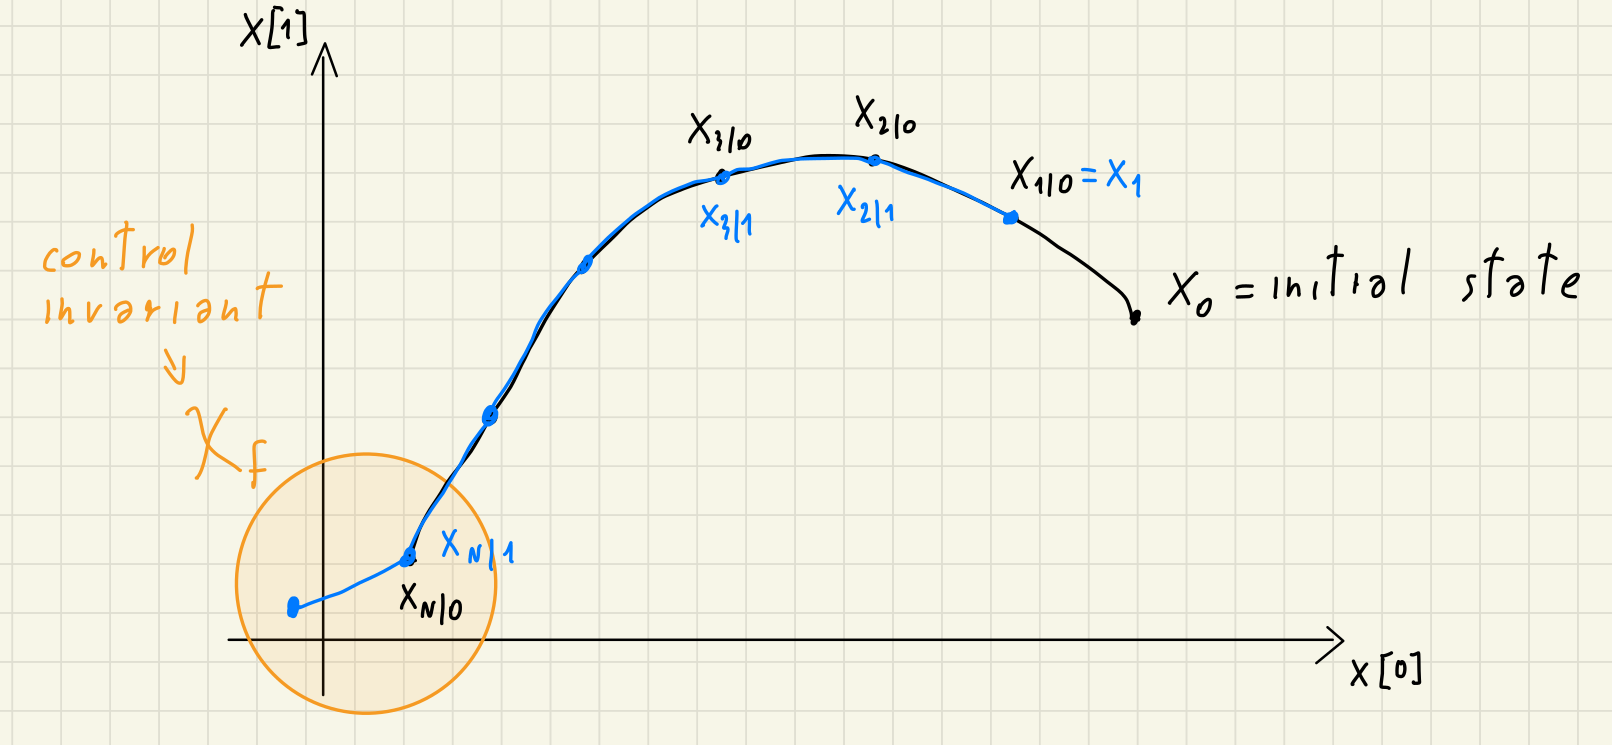
\includegraphics[width=.6\textwidth]{image0207}
\end{figure}

Example:
For a manipulator, set of zero velocity is control invariant (with zero velocity the manipulator remains in the same position with zero velocity i.e. you remain in the same state) if 
\begin{gather*}
\abs{g(q)}\le \tau^{max}\qquad\forall q \in[q^{min},q^{max}]\\
S=\{(q,0)|q^{min}\le q\le q^{max}, q\in\mathbb{R}^n\}
\end{gather*}
Which means that if the motor are sufficiently strong to compensate for gravity, then the set of possible states where the velocity is zero $S$ is control invariant.

\begin{center}
\textbf{How to compute the control invariant sets in general?}
\end{center}
\begin{itemize}
\item Hard problem for nonlinear systems (e.g. robot manipulator)
\item ``Maximal Output Admissible Set'' theory for linear systems. The same theory gives you some numerical algorithm to compute control invariant sets, but they only apply to linear systems.

Let us suppose that we have a system with linear dynamics:
\[x^+ = Ax\qquad y=Cx\]
And we have some constraints on the output (which are allowed to be nonlinear, and they can include state constraints and input constraints)
\[y\in\mathfrak{Y} = \{y\in\mathbb{R}^p: h_i(y)\le 0, i=1,...,s\}\]
The objective of the algorithm is to find a specific control invariant set, that is the maximum output admissible set:
\[O_{\infty} = \{x\in\mathbb{R}^n: h_i(CA^tx)\le 0, i=1,...,s, t=0,...,\infty\}\]
which is the set of all initial states $x$, s.t. if you start in $x$ the constraints on the output are always satisfied.
\end{itemize}

\subsubsection{Maximal Output Admissible Sets}
\begin{theorem}
If $A$ is Lyapunov stable, $h_i$ are continuous and they contain the \side{origin} (i.e. $h_i(0)\le0$) then:
\[O_{\infty} = O_{t^*} = \{x\in\mathbb{R}^n: h_i(CA^tx)\le 0, i=1,...,s, t\in\{0, ..., t^*\}\}\]
With the only difference that we can compute the set with a finite number of computation instead of infinity.
\end{theorem}
One possible way to compute $t^*$, even if it is not the best way, is to start with $t=0$ and compute $O_t$ until $O_{t+1}=O_t$.

This is theoretically fine but actually comparing $O_{t+1}$ to $O_t$ could be quite hard, so there is another way to do it:
\begin{enumerate}
\item Sove this problem for $i=1,...,s$:
\begin{align*}
\max_x J_i(x) &= h_i(CA^{t+1}x)\\
\text{s.t. } & h_j(CA^kx)\le 0\qquad j=1,...,s , k=0,...,t
\end{align*}
\item If $J_i^* < 0 \quad \forall i = 1,...,s$ then assign $t^* = t$.

Otherwise increment $t$ and repeat.
\end{enumerate}
What you are trying to do is similar to what we were trying to do with the first method, but the computation that you need to at each iteration is just s-optimization problems, where $s$ is the number of inequalities that define your constraints set, and what you are trying to do is to see if it is possible to violate one of the constraints at the time step  $t+1$ assuming that you satisfied the constraints at all the previous time steps.

If it is possible to do so, then you need to increase $t$ and keep going, whenever it is not possible to do so, it means that all constraints are satisfied and at that point you obtain $t^*$ and the algorithm stops.

\begin{center}
\textbf{What about control inputs?}
\end{center}


Fix $u= Kx$, which implies $x^+ = (A+BK)x$. Ultimately obtaining :
\[y = \M{I\\K}x\qquad\mathfrak{Y} = \mathfrak{X}\times\mathfrak{U}\]

\begin{theorem}
If $\mathfrak{X}_f$ is control invariant then the MPC is \side{persistently feasible}
\end{theorem}

Proof plan:
\begin{enumerate}
\item Given $X_f$ compute backward reachable sets $X_i$, i.e. set from which $X_f$ can be reached
\item Show that if $X_f$ is control invariant, then $X_i$ is control invariant $\forall i < N$
\item Show that if $X_1$ is control invariant, then the MPC is recursively feasible
\end{enumerate}
\begin{proof}
\begin{enumerate}
\item Given $x_n \in \mathfrak{X}_f = \mathfrak{X}_n$ define \side{backward reachable sets} recursively:
\[\mathfrak{X}_i = \{x\in\mathfrak{X}|\exists u\in\mathfrak{U}, \text{s.t. } f(x,u)\in\mathfrak{X}_{i+1}\}\]
By definition, if $x_N  \in \mathfrak{X}_N$ then $x_i\in\mathfrak{X}_i\qquad\forall i \in[0,N-1]$
\item If $X_f = \mathfrak{X}_N$ is control invariant, then $\mathfrak{X}_i$ is control invariant $\forall i$.

Assume $\mathfrak{X}_{i+1}$ is control invariant. This is true if and only if $\forall x \in \mathfrak{X}_{i+1}$, which implies that $\exists u \text{ s.t. } f(x,u)\in \mathfrak{X}_{i+1}$.

\begin{minipage}{.625\textwidth}
So from $\mathfrak{X}_{i+1}$ you can stay in $\mathfrak{X}_{i+1}$.

We know that $\mathfrak{X}_i$ contains all states from which you can reach $\mathfrak{X}_{i+1}$ so we infer:
\[\mathfrak{X_{i+1}}\subseteq \mathfrak{X}_i\]
Since from $\mathfrak{X}_i$ you can reach $\mathfrak{X}_{i+1}$, which is contained in $\mathfrak{X}_i$, we infer that from $\mathfrak{X}_i$ you can stay in $\mathfrak{X}_i$ which implies that $\mathfrak{X}_i$ is control  invariant.
\end{minipage}
\hfill
\begin{minipage}{.35\textwidth}
\centering
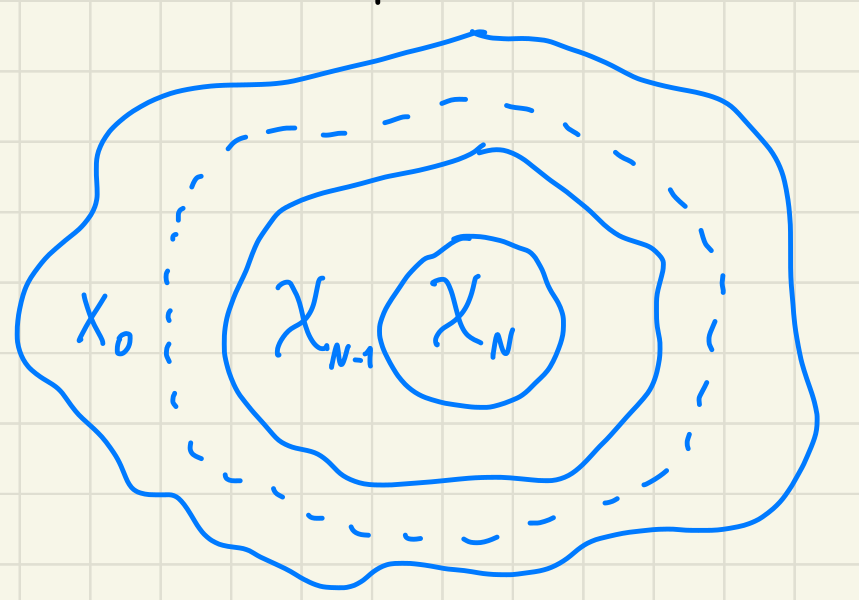
\includegraphics[width=.95\textwidth]{image0208}
\end{minipage}

By induction, starting from $\mathfrak{X}_N$ we can show that $\mathfrak{X}_i$ is control invariant $\forall i <N$.
\item We can show that 
\[\mathfrak{X}_i \subseteq \mathfrak{X}_0\]
Since the next state $x_1\in\mathfrak{X}_1$  then it is true that $x_1\in\mathfrak{X}_0$. However this is true if and only if the next MPC problem is feasible because $\mathfrak{X}_0$ is the set of all states from which MPC is feasible (by definition of $\mathfrak{X}_0$)
\end{enumerate}
\end{proof}
 
\subsection{Stability}
We can utilize Lyapunov Stability theorems to verify stability conditions of the MPC. Under this conditions, the key idea is to use the \side{Value function} (aka Optimal cost-to-go) as the \side{exponential Lyapunov function}.

The reason why it makes sense to use the Value function as a Lyapunov function is displayed in the following figure:
\begin{figure}[!h]
\centering
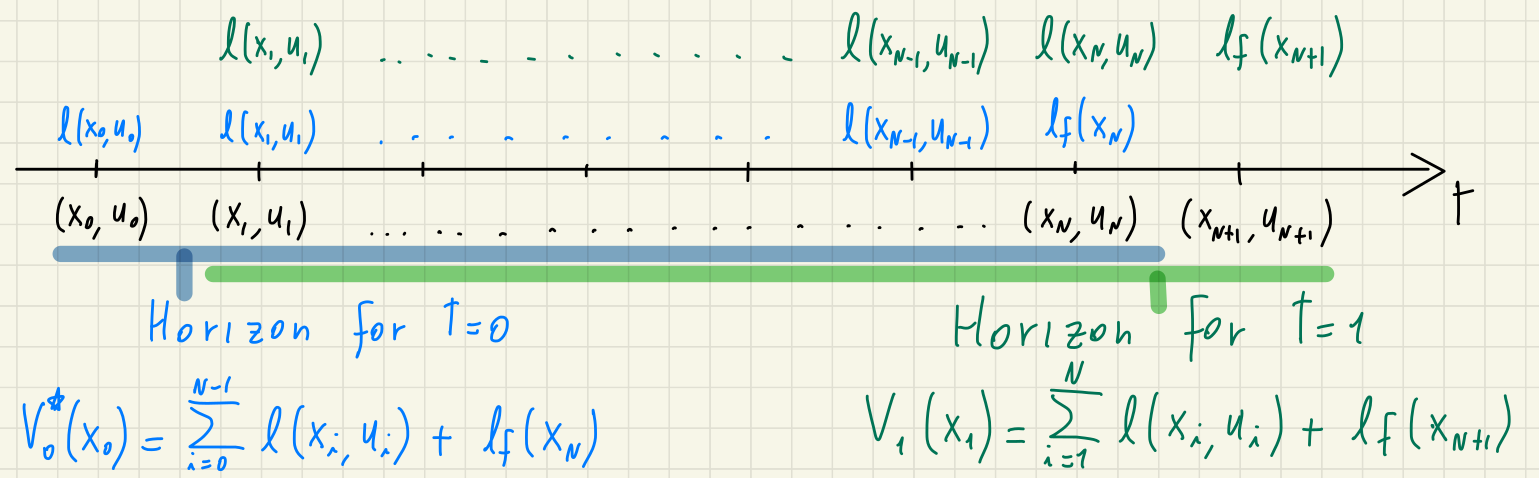
\includegraphics[width=\textwidth]{image0209}
\end{figure}
Along the time horizon over which we are optimizing and associated to each time step we have a cost which depends on the state and control at that time step.

So when we are at $t=0$ the horizon that we see, goes until time step $N$, whereas at $t=1$ the horizon that we see goes until time step $N+1$.

Imagine the cost that we will get in each of these two control problems that we solve:
\begin{itemize}
\item When we solve the first optimal control problem the cost will be:
\[V_0^*(x_0) = \sum_{i=0}^{N-1} l(x_i,u_i) + l_f(x_N)\]
with a summation of the running costs and the terminal cost
\item The same applies to the second optimal control problem starting at $t=1$:
\[V_1(x_1) = \sum_{i=1}^{N} l(x_i, u_i) + l_f(x_{N+1})\]
With the only difference being on the limit of the summation and the argument of the terminal cost.
\end{itemize}


We can notice that the intermediate running costs in the range $t\in[1,N-1]$ are equal: the only difference is in the terms:
\[l(x_0,u_0)\qquad l_f(x_N) \qquad l(x_N, u_N)\qquad l_f(x_{N+1})\]
Hence, we can write down the difference between the cost $V_1$ and the cost $V_0^*$ (the first two conditions of the Lyapunov function are easy to fullfill):
\begin{align*}
V_1(x_1) - V_0^*(x_0) &= \sum_{i=1}^{N}l(x_i,u_i) + l_f(x_{N+1}) - \sum_{i=0}^{N-1}l(x_i,u_i) - l_f(x_N)\\
&= \cancel{\sum_{i=1}^{N-1} l(x_i,u_i)} + l(x_N, u_N) + l_f(x_{N+1}) - l(x_0,u_0) - \cancel{\sum_{i=1}^{N-1} l(x_i,u_i)} - l_f(x_N)\\
&= l(x_N, u_N) + l_f(x_{N+1}) - l_f(x_N) - l(x_0, u_0)
\end{align*}
if i am able to prove that:
\[V_1(x_1) - V_0^*(x_0)  = l(x_N, u_N) + l_f(x_{N+1}) - l_f(x_N) - l(x_0, u_0) \le -\alpha_3 \norma{x_0}\qquad \forall x_N\in\mathfrak{X}_f\]
then the value function is an exponential Lyapunov function and I can use it to prove the stability of the origin for my system when it is controlled by the MPC.

One thing to notice is that $V_0^*$ is the \side{optimal value function} (i.e. the states and controls are optimal) , whereas for$V_1$ we assumed that we have used the values of the optimal state and control until $x_N$ and $u_N$ computed at the previous time step.

However, they may not be the optimal ones given that we are optimizing on a different horizon.

So by considering a non optimal value function we are taking a conservative approach: we are assuming that the trajectory will stay the same until the second to last time step.

This means that the condition that I want is a \side{sufficient condition}, but it is not necessary. So if it is satisfied I am sure that the system controlled by the MPC is stable.

\subsubsection{Stability Assumption}
\begin{enumerate}[label={\textbf{Ass. \#\arabic*}:}, leftmargin = 3cm]
\item The origin is an equilibrium point, the runnning cost at the origin is 0, the terminal cost at the origin is 0.
\[f(0,0)= 0\qquad l(0,0) = 0\qquad l_f(0) = 0\]
Note that assuming $f(0,0)$ is not restictive.
\begin{proof}
If we want to stabilize $x^* \ne 0$ s.t. $f(x^*, u^*) = x^*$, i.e. $x^*$ must be an equilibrium.

To achieve so we can define a new state $\bar{x}$, a new control $\bar{u}$ and new dynamics as follows:
\begin{align*}
\bar{x} &= x - x^*\\
\bar{u} &= u - u^*\\
\begin{dcases}
x^+ = f(x,u)\\
x^* = f(x^*, u^*)
\end{dcases}
&\qquad\Rightarrow\qquad
x^+ - x^* = f(\bar{x}+x^*, \bar{u} + u^*) - x^*\\
\bar{x}^+ &= \bar{f}(\bar{x}, \bar{u})
\end{align*}
So that $\bar{f}(0,0) = f(0+x^*, 0+u^*) - x^* = 0$
\end{proof}
\item The union of the state space and control space is a \side{closed set} (set that contains the boundaries):
\[\mathfrak{X} \times \mathfrak{U} \text{ is closed}\]
The terminal set is a \side{compact set} ($\approx$ closed + bounded set)
\[\mathfrak{X}_f \text{ is compact}\]

\item  For every state in the terminal constraint set there must exists a value of the control a collection of conditions must be respected.

Formally:
\[\forall x \in \mathfrak{X}_f\,\,\exists u \in \mathfrak{U} \text{ s.t.}\]
\begin{enumerate}
\item $\mathfrak{X}_f$ is control invariant
\[f(x,u)\in \mathfrak{X}_f\]
and the terminal cost decreases
\[l_f(f(x,u)) - l_f(x) \le - l(x,u)\]
\item There must exists 2 positive scalar, such that the running cost is lower bounded and the terminal cost is upper bounded, i.e.
$\exists \alpha_1, \alpha_f > 0$ s.t.
\begin{align*}
l(x,u)&\ge \alpha_1 \norma{x} & \forall x\in \mathfrak{X}_N, \quad \forall u\in\mathfrak{U}\\
l_f(x)&\le \alpha_f \norma{x} & \forall x \in \mathfrak{X}
\end{align*}
where $\mathfrak{X}_N$ is the set of states from which OCP has a solution
\end{enumerate}
\end{enumerate}
If these three assumptions are satisfied then $V_N^*(\cdot)$ is an exponetial Lyapunov function and therefore the origin is exponentially stable.


\begin{proof}
\[V_1(x_1) - V_0^*(x_0)  = l(x_N, u_N) + l_f(x_{N+1}) - l_f(x_N) - l(x_0, u_0) \le -\alpha_3 \norma{x_0}\qquad \forall x_N\in\mathfrak{X}_f\]
where:
\begin{itemize}
\item $l(x_N, u_N) + l_f(x_{N+1}) - l_f(x_N) \le 0$ 

by Ass \#3(a)
\item $- l(x_0, u_0) \le -\alpha_1\norma{x_0}$

by Ass \#3(b)
\end{itemize}
So we can be sure that the summation of these two will always be less that some negative function of $\norma{x_0}$
\end{proof}

\subsubsection{Example: Linear System}
Let us consider a linear system with dynamics:
\[x^+ = Ax + Bu\]
with some control constraints and state constraints:
\[u\in\mathfrak{U} \qquad x\in\mathfrak{X}\]
Whenever we have control and state constraints it is hard to find a global \side{Control Lyapunov Function (CLF)}.
For this reason we aim to find a local CLF inside a given region, called \side{invariant region} (given that it has the control invariant property).

Let us define the running cost the following quadratic function:
\[l(x,u) = \cfrac{1}{2} (x^TQx + u^TRu)\qquad\text{with } Q>0\,,\,R>0\] 
and then let us assume that the couple $(A, B)$ is \side{stabilizable} (i.e. it can be stabilized).
Under these conditions the Value function of unconstrained infinite horizon problem $\mathbb{P}_{\infty}^{un}$ is known and defined as:
\[V_{\infty}^{un}(x) = \cfrac{1}{2}x^TPx\]
where 
\[P =A_k^T P A_k + Q_k\]
with
\begin{gather*}
A_k\triangleq A+BK\qquad Q_k=Q+K^TRK \qquad u=Kx \qquad K=-(B^TPB+R)^{-1}B^TPA^T
\end{gather*}
In practice you can compute $P$ with an infinite summation of matrices
\[P = \sum_{i=0}^{\infty} (A_k^T)^iQ_kA_k^i\]
Of course this is not really practical (because you are doing an infinite summation), but since you are taking the power of a matrix that is stable (i.e. $A$), this matrix is going to zero as you keep summing. That means that at a certain point you can sto the summation and the error will be substantially small.

Knowing that this is the solution to the problem without the constraints what is  very often done is, we try to utilize it as a terminal cost in the problem with the constraint:
\[l_f(x) = V_{\infty}^{un}(x)\]
This makes sense given that we are looking for a local Control Lyapunov Function that is valid only inside a certain region, we can hope that if we are sufficiently close to the origin then the constraint won't play any role (in other words we expect that if we are sufficiently close to the origin the optimal choice won't be affected by the constraints) and that is what happens in practical application.

However, we still need to prove that using this particular choice of final cost, the stability assumption that we formulate for the Lyapunov Function are satisfied.
\begin{itemize}
\item \textbf{Terminal cost decrease}:
\[l_f(A_k x) + \cfrac{1}{2}x^TQ_kx - l_f(x)\le0\qquad\forall x \in \mathbb{R}^n\]
where:
\begin{align*}
l_f(x^+) &= l_f(Ax + Bu)&u=Kx\\
&=  l_f(Ax + BKx)&\\
&= l_f((A+BK)x) &\\
&= l_f(A_kx)&\\
&&\\
l(x, u) &= \cfrac{1}{2}(x^TQx + u^TRu)&u = Kx\\
&= \cfrac{1}{2}x^T(Q+K^TRK)x\\
&= \cfrac{1}{2}x^TQ_kx
\end{align*}

To verify that the assumption is verified, we substitute the uncontraint value function as the final cost, i.e.
\begin{align*}
l_f(A_k x) + \cfrac{1}{2}x^TQ_kx - l_f(x)&\le0\\
x^TA_k^TPA_kx + x^TQ_kx - x^TPx &\le0
\end{align*}
We obtained a summation of three pluriquadratic functions of the state, so this summation will always be negative if the matrix defining the quadratic form is negative semidefinitive
\[A_k^TPA_k + Q_k - P \le 0\]
which reminds us of the implicit definition of $P$, which is equal to zero.

We obtained that the terminal cost defined as the unconstrained value function can decrease and we also know that it decreases for the specific choice of the control input:
\[u=Kx\]
Note: $K$ could takes an arbitrary value, as long as the assumption are satisfied
\item \textbf{Terminal constraints}

Choose $\mathfrak{X}_f$ so that $u=Kx\in\mathfrak{U} \forall x\in\mathfrak{X}_f$ and $u=Kx$ makes $\mathfrak{X}_f$ will be positive invariant.

We can choose $\mathfrak{X}_f$ to be maximal invariant constrait admissible set for $x^+=(A+BK)x$.
\end{itemize}

In summary:
\begin{enumerate}
\item We can pick $\mathfrak{X}_f$ and $l_f(\cdot)$ such that:
\begin{itemize}
\item $\mathfrak{X}_f$ is control invariant
\item $\forall x \in \mathfrak{X}_f\,\exists u \in \mathfrak{U}$ s.t. $l_f(f(x,u)) - l_f(x) \le - l(x,u)$
\end{itemize}
\item We can pick $\mathfrak{X}_f = \{0\}$, i.e. picking the origin are your terminal constraint set.

Both conditions of the previous point are satisfied: the first one by definition given that the origin is control invariant, the second one is satisfied given that the terminal cost and the running cost at the origin are zero.

However this method results in a \side{small basin of attraction}, because you are constraining the terminal state to be in a set with just one point.
\item  We can pick $N$ ``large enough'' and set $l_f(x) = 0, \mathfrak{X}_f = \mathfrak{X}$. With nonlinear systems such as robots, that is what many people do (sadly).
\end{enumerate}

\subsubsection{Stability-Extensions}
\begin{enumerate}
\item \textbf{What if the system is time varying?}

So far we talked about stability of a point, i.e. the origin.

That is a very specific task for a robot to achieve, quite useless actually, because it means that you want the robot manipulator to stay still.

Tipically you want to do trajectory tracking and with the theory that we have looked at so far, we cannot really ensure stability for trajectory tracking because the running cost is not always the same but it depends on time.

In this case we can cast the trajectory tracking as regulation of time-varying system.

So the good news is that the theory can be extended to a time varying system:

Stability and recursive feasibility can still be ensured with time-varying $\mathfrak{X}_f$ and $l_f(\cdot)$.
\item \textbf{What if the cost function measures some sort of energy consumption?}

Another situation arises when the cost function measures some sort of energy consumption (quite common). In that case one of the assumptions that we took is not satisfied, i.e.
\[l(x,u) \ge\alpha \norma{x}\]
Because the running cost is not lower bounded anymore by the norm of the state, because the energy consumption does not depend on the norm of the state but tipically depends on both state and control.

In this situation, people rely on \side{Economic MPC theory} to prove and ensure stability of the system.  
\end{enumerate}

\subsection{Computation time}
In robotics, a lot of attention has been given to this issue: how do you make compilation faster?

One of the key idea that you can use to speed up computation is \side{warm start}, that goes as follow:

When you are solving the MPC optimal control problem for a given horizon from $0$ to $N$, and then at the next iteration you would have to solve another optimal control problem that looks quite a lot like the one we just solved (but we are shifting the horizon one step forward).

As a consequence, it seems really reasonable that the optimal solution won't change very much, because the problem and the solution are very similar. So what we can do is:

Take the optimal solution that you compute it at time $0$ and use it as an initial guess for the problem that you solve at the next time step. Since most of the time the optimal solution will be really similar then you have a good initial guess and the solver needs to take just a few iteration to converge to the optimal solution.

Formally:
\begin{itemize}
\item Shift trajectory back by 1 time step:
\[u^{guess}_k = u^*_{k+1}\]
\item Use zero as initial guess for last time step:
\[u_{N-1}^{guess} = 0\]
\end{itemize}

Another simple trick is that instead of iterating until convergence to a very small \side{convergence threshold}, do not iterate until convergence: at each iteration of the control loop just do one optimization iteration.

In this way you keep computation time to a minimum and you are show that you are always doing computation on the most recent information on the state of your robot (just do 1 Newton iteration).

There are many other ideas used to improve computation time, but these are the most general ones.

\subsection{Uncertainties in MPC}
Until now we did not really took into account \side{uncertainty}. We assumed that when we are at state $x$ we apply control $u$ and the next state will be $f(x,u)$.

In practice, what happens is that when we are at state $x$, we apply control $u$ and the new state will be $f(x,u) + noise$, because we do not have perfect knowledge of the dynamics, the actuators cannot really deliver the control input as you asked and you do not really know that your current state is $x$ because you have some uncertainty in your estimation due to \side{sensor noise}.

There are two main approaches to deal with uncertainties.
\subsubsection{Robust MPC}
In the \side{Robust MPC approach}, basically you consider the next state $x^+$ as a function of the state, the control input and the noise (with the noise bounded in a certain set), i.e.
\[x^+ = f(x,u,w)\qquad w\in \mathfrak{W}\]
As a consequence the generic constraint of the problem needs to be satisfied for every uncertainty that my happens
\[g(x,u,w)\le0\qquad \forall w\in W\]
In this way, i will always maintain a safety margin w.r.t. the constraint boundary and this safety margin is what allows us to ensure that the constraints will be satisfied for any possible uncertainty realization.

\subsubsection{Stochastic MPC}
Another approach is to define the uncertainty not simply bounded but it is a \side{stocastic uncertainty}, very often model with a \side{Gaussian distribution} with zero mean:
\[w ~ \mathfrak{N}(0,\Sigma)\]
In this case, since the uncertainty is Gaussian you cannot hope that the constraints will be satisfied for every possible value, given that it has a small probability of being infinitely large. So tipically, you impose that the probability of the constraint to be satisfied is greater than some value:
\[Pr[g(x,u,w)\le0] \ge 0.95\]


In general the Robust approach is easier to implement (mathematically speaking), but even though the stochastic approach is harder to implement it is \side{less conservative}.

Both these problem are well understood with \side{Linear dynamics}, i.e. there exists methods to find the solution for both approaches. with \side{Nonlinear dynamics}, some methods exist, but it is still ongoing research (as of now the methods either requires high computation effort or are extremely conservative).

\chapter{Reinforcement Learning}
\section{Introduction}
\side{Reinforcement Learning (RL)}, much like Optimal control, is a mathematical framework that allows us to solve optimal control problems.

In some sense is very similar to Optimal control, but with a very big difference: in Optimal control, you tipically assume to know the analytical/mathematical model of the system that you want to control, whereas in Reinforcement learning you don't.

Either you do not know the mathematical relation between input and state or you may assume that you have a simulator, but you do not have access to code.

Of course, since we have less information it is a much more difficult problem than optimal control, but they share the same structure and some of the key concepts (e.g value function).

A few differene between Reinforcement learning and Optimal control are:
\begin{itemize}
\item Optimal control was born in the control community, whereas reinforcement learning was born in the Computer Science community.
\item RL tries to find the \side{gloablly optimal policy}
\item RL assumes that the dynamics are unknown
\item Initally the community of RL was focused on problems in which the state and the control spaces were finite
\item RL uses different terminology than optimal control, with different names and symbols, even though they represent the same concept
\item tipically RL assumes the dynamics of the system to be stochastic (randomness on the state of the system)

However we will not take this assumption in this module (not a big deal), for sake of simplicity.
\item tipically RL literature focuses on optimizing over an infinite horizon
\end{itemize}

\section{Terminology comparison}

\begin{table}[!h]
\centering
\begin{tabularx}{\textwidth}{|X|X|}
\toprule
\textbf{Reinforcement Learning}&\textbf{Optimal control}\\
\toprule
State $s$& State $x$\\
Action $a$& Control $u$\\
Environment & Plant \\
Reward& Cost function\\
Return & Cost-to-go\\
Maximize&Minimize\\
Value function & Cost to go of a policy\\
Optimal Value function& Value function (Cost to go of the optimal policy)\\
\bottomrule
\end{tabularx}
\end{table}

\section{Framework: Markov Decision Processes (MDP)}
\side{Markov Decision Processes (MDP)} are used to describe the environment in Reinforcement Learning problems, which is assumed to be a \side{fully observable environment} and it has \side{Markov property}.

Markov property means that if you know the current state of the system than knowing the past states does not add any information.
The state tells you everything you know about the system.

Or in other terms: the future is independent on the past given the present.
\[\mathbb{P}(x_{t+1}|x_t) = \mathbb{x_{t+1}|x_1,...,x_t}\]
It can be immediately seen that the system is considered stochastic.

The motion of the state is defined by the \side{State transition probability} which the probability of going from one state $x$ to another state $x'$
\[\mathfrak{P}_{xx'} = \mathbb{P}(x_{t+1} = x' | x_t=x)\]
Since in classical Reinforcement Learning you assume that the size of the state space is finite, then you can collect together all the state transition probabilities in a big matrix, called \side{State Transition matrix}.
\[\mathfrak{P}=
\begin{bNiceArray}{ccc}
\mathfrak{P}_{11}&\Cdots&\mathfrak{P}_{1n}\\
\Vdots &\Ddots&\Vdots\\
\mathfrak{P}_{n1}&\Cdots&\mathfrak{P}_{nn}
\end{bNiceArray}\]
The sum of each row of the matrix will be 1. In deterministic systems $\mathfrak{P}$ contains only 0 and 1.

\subsection{Markov Process or Markov Chain}

A \side{Markov Process} is defined by a tuple $<\mathfrak{X}, \mathfrak{P}>$, where:
\begin{itemize}
\item $\mathfrak{X}$ is a finite set of states
\item $\mathfrak{P}$ is the \side{state transition probability matrix}
\end{itemize}
A Markov Process is also known as a \side{Markov Chain}
\missingfigure{33:16}

In particular the state transition probability matrix has the following property:
\begin{enumerate}
\item Since $\mathfrak{P}$ has all nonegative entries, and it is also \side{irreducible} (associated to a \side{strongly connected graph}), by using \side{Perron-Frobenius theorem} we know that:
\begin{itemize}
\item The largest (in nom) eigenvalue $r$ of $\mathfrak{P}$ satisfies the following inequalities:
\end{itemize}
\end{enumerate}


\appendix
\chapter{Numerical Integration}
\label{sec:num}

We are going to review Numerical Integration indipendently from Optimal Control.

Given an Ordinary Differential Equation (ODE)
\[\dot{x} = f(x,t)\]
with 
\[x(0) = x_0\]
Compute $x(t)\,\,\forall t \in [0, T]$.

If $f$ is \side{Lipshitz continuous} (i.e. the first derivative of the function are bounded) than this problem has an unique solution.

Moreover in $f$ has been omitted the dependency on $u(t)$ given that it is a function of time $t$ and/or $x$.

\section{Numerical Integration Methods}
\subsection{Explicit Euler}
\side{Explicit Euler} is the simplest numerical integration scheme based on the definition of the derivative as:
\[\dot{x} = \lim_{h\to 0} \,\cfrac{x(t+h) - x(t)}{h}\]
with $h$ ``small'' we can approximate $\dot{x}$ with the value on the rhs without the limit and write:
\[h\,\dot{x} \approx x(t+h) - x(t)\]
which means that 
\begin{empheq}[box=%
	\fbox]{gather*}
x(t+h) \approx x(t) + h\,f(x,t)
	\end{empheq}

\missingfigure{1:16:25}
So the key assumption of the Explicit Euler is to take $h$ sufficiently small in order for it to work but the methods does not specify exactly how small it must be the step. However taking $h$ small means that it will be computationally expensive.

Moreover it is not very accurate (first order method).

\subsection{Mid-Point Method}
The \side{Mid-Point Method} is slightly better than the Explicit Euler. 

You take a first step to reach the middle of the time step, you look at the value of $\dot{x}$ in the middle and this is the value that you use in the whole time step.

So you go back and you integrate the time step using the value of $\dot{x}$ that you computed in the middle of the step:
\begin{empheq}[box=%
	\fbox]{align*}
k_1 &= f(x_0, t_0)\\
k_2 &= f\left(x_0 + \cfrac{h}{2}\,k_1, t_0 + \cfrac{h}{2}\right)\\
x_1 &= x_0 + h\,k_2
\end{empheq}

\missingfigure{1:16:25}

\begin{enumerate}
\item Use the slope in the middle of the step to integrate forward
\item Estimate $x\left(t_0 + \cfrac{h}{2}\right)$ with the slop at $t_0$
\item Second order method (order 2)
\item Need 2 function evaluation for each step
\end{enumerate}

The theory that allows us to state that almost always the midpoint method is better than explicit Euler is the theory of numerical integration scheme.

\subsection{Runge-Kutta Methods}
The Euler method and midpoint method are both specific cases of \side{Runge-Kutta method}.

The RK methods are based on the following equations:
\begin{empheq}[box=%
\fbox]{align*}
x_{n+1} &= x_n + h\,\sum_{i=1}^q \,b_i\,k_i\\
k_i &= f\left(x_n\,+\,h\sum_{j=1}^q\,a_{ij}\,k_j , t_n + c_i\,h\right)
\end{empheq}
where:
\begin{itemize}
\item $q\,\,$ is the order of the method (not to be confused with the consistency order of the method)
\item For $q = 1$ we recover Euler by setting ($b_1 = 1, a_{11} = 0, c_1 = 0$)
\item The Mid-point method is an RK method of order $q = 2$
\item If $a_{ij} = 0\,\, \forall j\ge i$ the method is called \side{explicit method}.

Otherwise the method is called \side{implicit method} (need to solve system of equations because to compute $k_i$ you need to know the value of other $k$ that are all interdependent).
\item For $q > 1$ there exist many versions of the same order.
\item the term $\sum_{i=1}^q\,b_i\,k_i$ is an approximation of $\dot{x}$ with an weighted average of $k_i$, with weights $b_i$.

Where 
\[\sum b_i = 1 \qquad b_i \ge 0\]
\end{itemize}

Therefore to define a RK method you need all the values of parameter $a, b$ and $c$. Tipically these parameters are stored in a so called \side{Butcher Tableau}.

\[
\begin{NiceArray}{c|ccc}
c_1& a_{11}&\Cdots & a_{1q}\\
\Vdots &  \Vdots& \Ddots& \Vdots\\
c_q& a_{q1} & \Cdots & a_{qq}\\
\midrule
& b_1 &\Cdots&b_q
\end{NiceArray}
\]
\begin{itemize}
\item Once you have this tableau you have uniquely defined the RK method
\item Most common explicit RK4 method and takes the form
\begin{empheq}[box=%
\fbox]{align*}
k_1 &= f(x_n,\,t_n)\\
k_2 &= f\left(x_n + \cfrac{1}{2} h\,k_1, t_n + \cfrac{1}{2}\,h\right)\\
k_3 &= f\left(x_n + \cfrac{1}{2} h\,k_2, t_n + \cfrac{1}{2} h\right)\\
k_4 &= f(x_n + h\,k_3, t_n\,+\,h)\\
x_{n+1} &= x_n + \cfrac{h}{6} (k_1 + 2\,k_2 + 2\,k_3+k_4)
\end{empheq}
and it can be uniquely defined by the Butcher Tableau:
\[
\begin{NiceArray}{c|cccc}
0& \\
\sfrac{1}{2}& \sfrac{1}{2} & \\
\sfrac{1}{2}& 0 & \sfrac{1}{2}\\
1 & 0 & 0 & 1\\
\midrule
& \sfrac{1}{6} &\sfrac{1}{3}&\sfrac{1}{3}&\sfrac{1}{6}
\end{NiceArray}
\]
The main reason this method is so common comes from the fact that it draws the limit for which you get a method that has the same consistency order of the order of the RK scheme (i.e. for $p\ge5 \,\nexists \text{method with } q=p$).
\end{itemize}
\missingfigure{comparison of RK methods 19:11}
\section{Properties of Integration Schemes}
Definitions:
\begin{itemize}
\item{\makebox[5cm]{Integrator output:\hfill} $\hat{x}(t, t_0, x(t_0))$}
\item{\makebox[5cm]{Exact trajectory:\hfill} $x(t)$}
\item{\makebox[5cm]{Local integration error:\hfill} $e(t) = x(t) - \hat{x}(t, t-h, x(t-h))$}
\item{\makebox[5cm]{Global integration error:\hfill} $E(t) = x(t) - \hat{x}(t, t_0, x(t_0))$ }
\end{itemize}
Now that we have defined these two error we can talk about the properties of integration schemes which are:
\begin{enumerate}
\item \side{Convergence}.

Convergence is the basic properties that ensures that as the time step that you use for integration goes to zero the global error should go to zero as well:
\[\lim_{h\to0} \,E = 0\]
It is not a very difficult property to achieve. Basically all the integration methods have this property.
\item \side{Consistency order} p.

Tells you how quickly the error goes to zero. In particular it is formulated using the local error.
In particular the limit of the local error should go to zero as a polynomial of the time step:
\[\lim_{h\to0}\,e=O(h^{p+1})\qquad p>0\]
So when we refer to a method order 1 or 2 we refer to the value of p on the above definition.
\item \side{Stability}.

There is no clear definition of stability.  But we can approximately define it as the global error remains bounded as we keep integrate ($t\to\infty$)
\end{enumerate}

From this definitions we can now quantify the performance of each method through the notion of consistency order.
\begin{itemize}
\item The local error for Explicit Euler takes the form:
\[e(t) \triangleq x(t+h) - \hat{x}(t+h, t, x(t)) = x_{n+1} - \hat{x}_{n+1}(x_n) = e_{n+1}\]
where 
\[x_n \triangleq x(t_n)\]
So we can reformulate the expression as:
\[\hat{x}_{n+1} = x_n + h\,f(x_n, t_n)\]
Let us express $x_n$ with a Taylor series around $x_n$:
\[x_{n+1} = x_n + h\,\dot{x}_n + O(h^2)\]
Whatever remains is something in the order of $h^2$.
And Finally we can compute the error with the expression above:
\begin{align*}
e_{n+1} &= x_{n+1} - \hat{x}_{n+1}\\
&= \cancel{x_n} + \cancel{h\,\dot{x}_n} + O(h^2) - \cancel{x_n} - \cancel{h\,f(x_n,t_n)}\\
&= O(h^2)
\end{align*}
So this means that the method is of order 1 (i.e. $p = 1$)

\item The local error for Mid-point method takes the form:
\[e(t) = x(t+h) - \hat{x}(t+h, t, x(t)) = x_{n+1} - \hat{x}_{n+1}(x_n)\]
where
\begin{align*}
k_1 &\triangleq f(x_n, t_n) = \dot{x}_n\\
\hat{x}_{n+1} &= x_n\,+h\,f\left(x_n+\cfrac{h}{2}\,k_1, t_n + \cfrac{h}{2}\right)\\
f &= \dot{x}\\
\dot{f} &= \left(\pd{f_n}{x_n}\,\td{x_n}{t_n} + \pd{f_n}{t_n}\right) = \ddot{x}
\end{align*}
Let us express $x_{n+1}$ with the Taylor series around $x_n$:
\[x_{n+1} = x_n + h\,\dot{x}_n + \cfrac{h^2}{2}\,\ddot{x}_n + O(h^3)\]
And let us express $f(x_n+\cfrac{h}{2}\,\dot{x}_n, t_n + \cfrac{h}{2})$ with the Taylor series around $(x_n, t_n)$:
\begin{align*}
f\left(x_n+\cfrac{h}{2}\,\dot{x}_n, t_n + \cfrac{h}{2}\right) &=f(x_n, t_n) + \pd{f_n}{x_n}\,\cfrac{h}{2}\,\dot{x}_n \, +\, \pd{f_n}{t_n}\,\cfrac{h}{2} + O(h^2)\\
&= \dot{x}_n + \cfrac{h}{2}\,\ddot{x}_n + O(h^2)
\end{align*}
We can finally write the error using the expressions above:
\begin{align*}
e_{n+1} &= x_{n+1} - \hat{x}_{n+1} \\
&= \cancel{x_n} + \cancel{h\,\dot{x}_n} + \cfrac{h^2}{2}\,\ddot{x}_n\,+O(h^3) - \left(\cancel{x_n}\,+ h\,\left(\cancel{\dot{x}_n}\,+\cfrac{h}{2}\,\ddot{x}_n + O(h^2) \right)\right)\\
&= O(h^3)
\end{align*}
So this means that the method is of order 2 (i.e. $p = 2$)
\end{itemize}
\chapter{Lyapunov Stability}
\section{Exponential Lyapunov functions}
Stability of a method can be proved using \side{Lyapunov functions}, which are one of the main tools to prove stability of nonlinear systems.

\textbf{Def:} A set $S$ is \side{positive invariant} if $\forall x \in S$ the next state is also inside the set, i.e. $f(x) \in S$.

In other terms if $x$ starts in $S$ then it stays inside $S$.\newline

\textbf{Def:} Suppose $\mathfrak{X}$ is positive invariant, a value function $V: \mathbb{R}^n \to \mathbb{R}^+$ is an \side{exponential Lyapunov function} if $\exists \alpha_1, \alpha_2, \alpha_3 > 0$ (three positive constants) s.t. $\forall x \in \mathfrak{X}$, the following conditions are satisfied:
\begin{align*}
V(x)&\ge \alpha_1 \norma{x}\\
V(x)&\le \alpha_2 \norma{x}\\
V(f(x))-V(x)&\le -\alpha_3\norma{x}
\end{align*} 
Which means that the value function needs to be 
\begin{itemize}
\item lower bounded
\item upper bounded 
\item decreasing exponentially along the trajectory of $x$.
\end{itemize}

The following theorem specifies when the system is \side{exponentially stable}, i.e.:
\[\norma{x_k}\le c\,\gamma^k\,\norma{x_0} \quad \text{for some } c >0 \text{ and } \gamma\in[0,1]\]
\begin{theorem}
If $\exists$ a Lyapunov function then the \side{origin} (state $x=0$) of the system is exponentially stable in the set $\mathfrak{X}$.

If $\mathfrak{X} = \mathbb{R}^n$ then the origin is globally exponentially stable.
\end{theorem}

Even though this theorem can be applied to stabilize the origin, it can be extended to an arbitrary state.



\clearpage
\addcontentsline{toc}{chapter}{{Index}}
\listoftodos[Index]

\clearpage
\chapter*{Bibliography}
\addcontentsline{toc}{chapter}{{Bibliography}}
\printbibliography[heading=bibempty]

\end{document}